\documentclass{report}


% General imports:
\usepackage[utf8]{inputenc}
\usepackage[T1]{fontenc}	% For using icelandic Thorn character
\usepackage{amsmath}
\usepackage{graphicx}

% Support for spanish:
\usepackage[spanish]{babel}

% Imports for images
\usepackage{caption}
\usepackage{subcaption}
\usepackage{wrapfig}

% Imports for euro symbol support
\usepackage[official]{eurosym}
\DeclareUnicodeCharacter{20AC}{\euro{}}

% Other imports:
\usepackage{indentfirst} % Indent first paragraph
\usepackage[nottoc,numbib]{tocbibind} % Add bibliography to table of contents
\usepackage{url}	% Cite URLs

% Formatting margins of the pages:
\usepackage[top=2.3cm, bottom=2.29cm, left=2cm, right=2cm]{geometry}

% Import for headers
\usepackage{fancyhdr}

% Definitions of important data
\renewcommand{\author}{David Estévez Fernández\\Enrique Fernández Rodicio\\Javier Isabel Hernández}
\renewcommand{\title}{??}
\newcommand{\department}{Máster Universitario de Robótica y Automatización\\Robots Móviles}
\newcommand{\teacher}{Ramón Barber Castaño}

% Define a command for comments
\usepackage{color}
\newcommand{\comment}[1]{\textbf{\color{red} #1}}

% Each chapter will have its own header
%\newcommand{\headchapter}[1]{\chapter{#1}\rhead{#1}}

% Each section will have its own header
%\newcommand{\headsection}[1]{\section{#1}}\rhead{#1}}

% Change 'Chapter' to something more logical
\renewcommand{\chaptername}{}

% This is for writing algorithms on pseudocode (nicely)
\usepackage{algorithm}
\usepackage[noend]{algpseudocode}

% This is used for adding appendices:	
\usepackage[toc,page]{appendix}

\begin{document}

%%%% FRONTPAGE %%%%%%%%%%%%%%%%%%%%%%%%%%%%%%%%%%%%%%%%%%%%%%%%%%%%%%%%%%%%%%%%
\newcommand{\frontpage}[4]
{
\begin{center}

\includegraphics[width=0.25\textwidth]{./images/uc3m.jpg}\\[2cm]
\textsc{\LARGE Universidad Carlos III de Madrid}\\[0.5cm]
\textsc{\Large #1}\\[3cm]


% Title
{\huge \bfseries{#2}\\[7cm]}


% Author and supervisor
\begin{minipage}{0.35\textwidth}
\begin{flushleft} \large
\emph{Autores:}\\
#3\\
\end{flushleft}
\end{minipage}
\begin{minipage}{0.4\textwidth}
\begin{flushright} \large
\emph{Profesores:}\\
#4
\end{flushright}\end{minipage}\vfill

% Bottom of the page
{\large \today}

\end{center}
%
\newpage
%
}

\frontpage{\department}{\title}{\author}{\teacher}

% Adding some header text on top of the page:
\lhead{}
\chead{}
\rhead{\title}
\pagestyle{fancy}


%%%%%%Table of contents%%%%%%%%%%%%%%%%%%%%%%%%%%%%%%%%%%%%%%%%%%%%%%%%%%%%%%%%
\tableofcontents
\newpage

%%%% Different Sections %%%%%%%%%%%%%%%%%%%%%%%%%%%%%%%%%%%%%%%%%%%%%%%%%%%%%%%
\chapter{Introducción}
\label{introducción}

El objetivo de este trabajo es aplicar los conocimientos adquiridos tanto en esta asignatura como a lo largo del Máster en el desarrollo de un caso práctico de estudio. Para ello, en esta memoria se presenta el proyecto Beerbot (Beer Extracting Environment Robot), un sistema compuesto por un robot móbil y una cámara aérea situada sobre el escenario. La camará se encargará de tomar imagenes del entorno, estas se procesarán para obbtener las características deseadas y posteriormente un algoritmo de planificación de trayectorias generará un camino que permita al robot cumplir su misión evitando obstáculos y siguiendo la ruta más directa. La tarea programada es recoger una lata en algún punto del entorno, y devolverla al punto inicial.\\

Este trabajo se divide en los siguientes apartados. Después de esta breve introducción, se llevará a cabo un breve estudio acerca de la navegación autónoma para robots móviles acerca de la impresión 3D, las diferentes tecnologías existentes y del uso de técnicas de impresión 3D en la fabricación de estos robots.\\

En la siguiente sección se pasará a hablar del proyecto Beerbot en sí. Se dividirá en tres subapartados. En el primero se presentará el proyecto y los objetivos a conseguir, además de mostrar el entorno de pruebas empleado. El siguiente apartado tratará sobre el hardware empleado, es decir, se comentará el diseño y funcionamiento del robot y el modelo de cámara con el que se va a trabajar. Por último, el último subapartado tratará acerca del software desarrollado, que se puede clasificar en trés etapas. La primera de ellas consiste en el procesamiento de las imagenes tomadas por la cámara, de las que se extraerán los obstáculos presentes en el entorno, la posición y orientación del robot y la posición de la lata (al ser cilíndrica, la orientación de la lata es irrelevante). La segunda etapa es la planificación de la trayectoria. Se usará un planificador probabilístico para muestrear el espacio libre y un método de resolución de grafos para encontrar el camino. Por último, la tercera etapa consiste en el mecanismo de control del robot, que transformará los datos extraídos del planificador en comandos de velocidad para las ruedas, y que se encargará también de asegurar que el robot no se desviará de la ruta seleccionada.\\

Por último, se mostrarán imagenes del sistema en funcionamiento y se comentarán los resultados obtenidos, además de mostrar algunas posibles mejoras que se han considerado pero no se han podido llegar a implementar, antes de cerrar este trabajo con una conclusión final.\\

\chapter{Estado del arte}
\label{estado del arte}

En esta seccion se realizara un breve estudio 

\section{Navegación de robots autónomos}
\label{navegacion_de_robots}

Un robot móvil es aquella máquina automática que puede moverse en un determinado entorno. En función de la forma en la que se mueva se pueden dividir en diferentes categorías: robots rodantes (emplean ruedas para moverse), andantes (emplean dos o más extremidades para desplazarse), reptantes (se arrastran por el suelo), nadadores, voladores…\\

En el campo de la robótica móvil, se conoce como navegación al guiado de un robot que parte de un punto inicial, a través de un entorno en el que existen ciertos obstáculos a evitar, para alcanzar el punto final deseado. Para que se pueda cumplir con un cierto éxito esta tarea, es necesario poder resolver cuatro grandes problemas: Generar un mapa, localizar al robot en el, generar una trayectoria que una los puntos inicial y final y, por último, ser capaz de seguir esa trayectoria sin desviarse.\\

En primer lugar, se necesita proporcionar al robot un mapa del entorno que posea una precisión adecuada. Este puede haber sido realizado de antemano, o generado por el propio robot, empleando para ello los diversos sensores con los que cuenta, al mismo tiempo que avanza. Esta técnica es conocida como Simultaneous Localization And Mapping, o SLAM, que busca que el robot pueda ser capaz de generar el mapa de su entorno y, al mismo tiempo,  pueda localizarse con éxito dentro de ese mapa. De entre todas las técnicas empleadas para su solución, las más efectivas son las basadas en técnicas probabilísticas, que parten del teorema de Bayes, para poder tener en cuenta las distintas fuentes de incertidumbre que van apareciendo a lo largo del problema. Los principales algoritmos en este campo son el Filtro Extendido de Kalman, los mapas de ocupación de celdillas o la solución factorizada del filtro de Bayes.\\

A continuación, el robot debe ser capaz de localizarse dentro del mapa del entorno. Si para generar dicho mapa se empleó la técnica de SLAM, el punto anterior y este se resuelven de forma simultánea. Si el mapa fue generado de forma externa, debe emplearse un sistema que permita al robot conocer su posición. Por lo general, existen tres familias de algoritmos para esta tarea, aquellos basados en el concepto de probabilidad bayesiana, aquellos que plantean la localización del robot como la solución a un problema de optimización, y aquellos que mezclan conceptos de los dos tipos anteriores, conocidos como métodos híbridos.\\

El teorema de Bayes establece que la probabilidad que la probabilidad de que se dé un suceso aleatorio A conociendo que otro suceso B ya ha ocurrido depende de la distribución de probabilidad condicional de B si A ha ocurrido y de la distribución de probabilidad marginal de A. Aplicado a la localización de robots móviles, se calcula la probabilidad a posteriori asociada a una posible posición del robot dentro del espacio de soluciones del problema con los datos extraídos de la odometría y de los sensores y, a continuación, partiendo del paso anterior, se estima la posición futura del robot. Dentro de esta familia, destacan los métodos de localización de Markov y el filtro de Kalman, aunque este último no permite obtener la posición del robot, simplemente sirve para mantener localizado al robot durante el movimiento.\\

En cuanto a los métodos de optimización, trabajan con una función de coste que asigna a cada posible posición del robot un valor de coste. Una vez se tiene definida dicha función, se usa uno de los métodos de resolución de problemas de optimización, como pueden ser los algoritmos evolutivos, para tratar de encontrar la solución cuyo valor de coste sea mínimo. En bastantes casos, el coste es la medida que representa la diferencia que hay entre las medidas de los sensores del robot y de las medidas estimadas que se obtendrían si el robot se encontrase en esa posición.\\

Una vez hecho esto, el robot debe ser capaz de elegir una ruta libre de obstáculos para poder desplazarse desde el punto inicial al punto final. Para resolver este problema, se puede tener en cuenta las características de movimiento del robot a emplear o se puede buscar una solución basada simplemente en el mapa del entorno  y los puntos inicial y final. La planificación se puede plantear de dos maneras, de forma explícita, construyendo el espacio libre, aunque estó puede ser excesivamente costoso computacionalmente hablando, o muestreando el espacio libre, sin llegar a definirlo por completo, lo que es suficiente para encontrar u buen camino, usando un número suficiente de muestras.\\

Un planificador es completo si es capaz de encontrar un camino, en caso de que exista, en un tiempo finito. Los planificadores completos de resolución garantizan una solución si la resolución de la rejilla con la que se representa el espacio libre es lo suficientemente alta. Por último, los planificadores probabilísticos, como el método de Monte Carlo, ofrecen una mayor probabilidad de encontrar el camino cuantas mas iteraciones se realicen.\\

En general, hay cinco tipos de planificadores. Los planificadores basados en rejilla representan el espacio de configuraciones como una cuadrícula, donde cada punto de esta representa una posible configuración del robot. Para encontrar el espacio libtre, se comprobará si el camino entre dos celdas contiguas está despejado, y en caso afirmativo, se añadirá al conjunto de puntos por los que puede pasar el robot. Por último, se usa un método de resolución de grafos para encontrar el camino. Este método no es muy recomendable para entornos muy grandes o no estáticos, ya que la rejilla crece de forma exponencial con el tamaño del escenario, y en caso de que algo cambie, hay que volver a calcular el espacio lbre .\\

Los planificadores basados en intervalos son similares a los que se acaban de ver, solo que en este caso, el tamaño de las celdas no tiene por que ser uniforme. Estas celdas se dividen en dos subconjuntos, $X^-$ y $X^+$, donde $X^-$ es el espacio por el que el robot se puede mover sin problemas, mientras que $X^+$ es el espació máximo del cual no se puede salir. Al igual que antes, se usa un método de resolución de grafos para encontrar la trayectoria, que tiene que estar contenida en $X^+$ y ser factible en $X^-$. Dada su similitud con los planificadores basados en rejilla, también comparte uno de sus problemas, y es que este método tampoco es muy recomendable en entornos muy grandes.\\

Los planificadores geométricos representan tanto los obstáculos como el robot como polígonos. Después, con grafos de visibilidad o descomposición de celdas, se calcula el camino para que el robot pueda pasar entre los obstáculos.\\

Los planificadores basados en campos de potencial representan el entorno como un campo de potencial, donde el objetivo definido para el robot genera una fuerza de atracción, mientras que los obstáculos generán una fuerza de repulsión. Son algoritmos muy poco costosos desde el punto de vista computacional, pero por otra parte, pueden quedarse atrapados en mínimos locales, aunque se han desarrollado métodos dentro de esta familia que solucionan este problema, como es el caso del Fast Marching.\\

Por último, los planificadores basados en muestreo son bastante efectivos para entornos de muchas dimensiones, son fáciles de implementar y además, son planificadores completos, por lo que siempre encontrarán un camino, si este existe. Se distribuyen una serie de muestras por el entorno (existen diferentes aproximaciones para esto), asegurandose de que no caigan dentro de ningún obstáculo. Después, se unen aquellos puntos entre los que el robot puede moverse sin colisionar. Por último, se usa algún método como el $A^*$ o el Dijkstra para encontrar el camino. Con estos planificadores, el hecho de no encontrar un camino, no significa que no exista, ya que lo mismo si se aumenta el número de muestras se podría obtener una trayectoria. Dentro de esta familia se encuentran los algoritmos PRM, o Probabilistic Road Map o los Rapidly-expanding Random Trees (RRT).\\ 

Por último, el robot debe ser capaz de seguir la ruta que planificó anteriormente. Esto supone resolver la forma de adecuar dicha ruta a los parámetros que caracterizan el movimiento del robot (en caso de no haberlo hecho a la hora de panificar la ruta), además de poder mantener un seguimiento de su localización a lo largo del desplazamiento. Además, debe seguir recibiendo información del entorno a través de los sensores para poder reaccionar adecuadamente a la aparición de un obstáculo imprevisto.\\

En este trabajo se ha optado por una alternativa poco ortodoxa en cuanto al método para extraer el mapa y la localización del robot, ya que esto se consigue mediante una cámara externa que toma imágenes del entorno y las procesa para extraer los datos deseados. Para la planificación, se ha empleado un algoritmo basado en el muestreo, en concreto el PRM, y el seguimiento de la trayectoria se realiza de forma directa, reorientandose respecto al siguiente punto del camino cada vez que se avanza un poco.\\     
\section{Impresion 3D aplicada a la robotica}
\label{impresion_3D}
\section{Vision por computador}
\label{vision_por_computador}
\chapter{Desarrollo del proyecto}
\label{desarrollo}

\section{Introducción al proyecto Beerbot}
\label{introduccion_desarrollo}

En esta sección se presenta la parte central del trabajo, el proyecto Beerbot, acrónimo de Beer Extraction Experimental Robot. Se trata de un sistema formado por un robot móvil con una pinza y una cámara situada sobre el escenario. La cámara se conectará con un ordenador, que será el encargado de ejecutar el algoritmo desarrollado, desde el procesamiento de la imagen a la planificación de la trayectoria y el control de alto nivel del robot. Este ordenador se comunicará con el microcontrolador del robot a través de un módulo bluetooth, enviándole la velocidad de giro de cada rueda.\\

\begin{figure}[H]
        \centering
        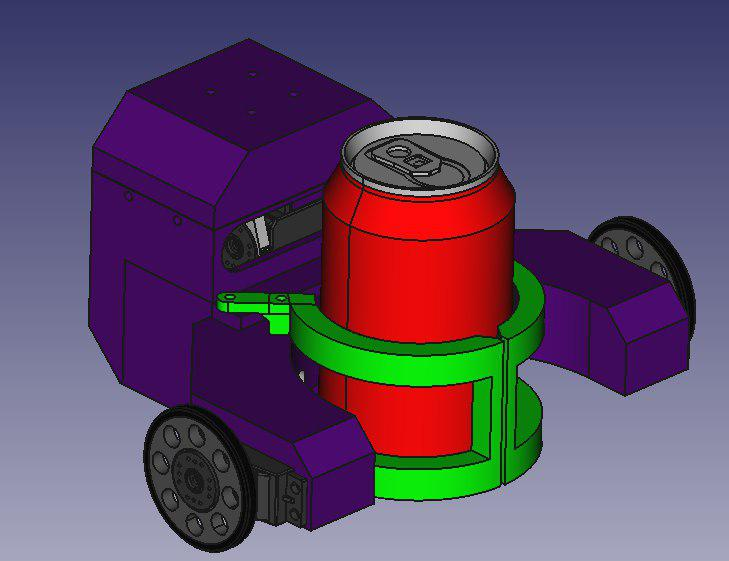
\includegraphics[width=0.4\textwidth]{images/robot.jpg}
        \caption{Modelo 3D del robot}
        \label{fig:robot}
\end{figure} 

\subsection{Objetivos}

El objetivo principal de este proyecto es desarrollar un robot que sea capaz de navegar por un entorno con obstáculos estáticos para localizar una lata, recogerla con la pinza y llevarla al punto inicial. Para ello se trabajará con algoritmos de procesamiento de imágenes, algoritmos de planificación de trayectorias, e impresión 3D, para la fabricación del robot.\\

Además de este objetivo, con este trabajo también se pretende diseñar una aplicación real y física que permita poner en práctica los conceptos adquiridos no solo en la asignatura en sí, si no a lo largo del máster. Se han llevado a cabo otros proyectos acerca de planificación, pero en entornos simulados, por lo que la fabricación del robot y el uso de un entorno real son la parte clave, ya que con esto se podrá estudiar como las características del entorno afecta a los resultados obtenidos.\\
 
Respecto a la parte de procesamiento de imágenes, el hecho de tener un escenario con iluminación no controlada obligará a tener que explorar diferentes alternativas para combatir los cambios de iluminación y poder conseguir los resultados esperados, especialmente en la etapa de segmentación de la imagen. Por otra parte, a diferencia de las simulaciones, el robot presentará errores de posición que será necesario corregir añadiendo un mecanismo de seguimiento de la trayectoria, para asegurarse que se llegue al punto al que realmente se está tratando de llegar.\\
 
\subsection{Funcionamiento del sistema}

El sistema funciona de la siguiente manera. El robot se sitúa en el escenario elegido, en un punto cualquiera. La cámara aérea captura una imagen del escenario, que se procesa para extraer de ella los obstáculos presentes en el entorno, la posición y orientación del robot y la posición del objetivo, es decir, la lata. Todos estos datos se envían al algoritmo de planificación, que muestrea el espacio libre por el que puede pasar el robot y calcula la ruta óptima por la que se pueda alcanzar el objetivo sin colisionar con los obstáculos. Conociendo los puntos por los que pasa la trayectoria, se va controlando la posición del robot en cada instante y se convierte la diferencia entre dicha posición y el siguiente punto del camino a comandos que le indiquen al robot la velocidad que debe llevar cada rueda. Una vez se alcanza una posición cercana a la lata, se abre la pinza, se coge la lata y el robot hace el mismo camino en la otra dirección (se supone que al ser un entorno estático, la trayectoria óptima debería seguir siendo la misma, además de simplificar el proceso, al ahorrarse un ciclo de planificación) hasta llegar al punto del que había partido, donde dejará la lata. En la siguiente sección de la memoria se comentarán más en detalle las diferentes partes del sistema.\\

\subsection{Escenario a utilizar}

Se va a trabajar sobre una pista cuadrada desarrollada para el concurso de robótica humanoide CEABOT. Tiene unas medidas de 2mx2m y un suelo de color verde, que facilita las tareas de segmentación. Para los obstáculos, se han utilizado objetos diversos que se han encontrado en la zona de trabajo, ya que era lo que se tenía a mano. Además con esto se consigue otra cosa: mostrar que no es necesario que los obstáculos tengan un color, tamaño o forma determinada, ya que se pueden detectar como tal sin problema. En cuanto a la lata, tendrá un tamaño estándar, pero no es necesario que tenga un color determinado, lo que permite que el sistema no esté limitado a un único tipo de objetivo. En cuanto a la cámara, se han utilizado dos listones rígidos unidos por un cable como estructura para soportarla. En la figura \ref{fig:escenario} se puede observar el escenario utilizado, el robot, y diversos objetos usados como obstáculos.\\

\begin{figure}[H]
        \centering
        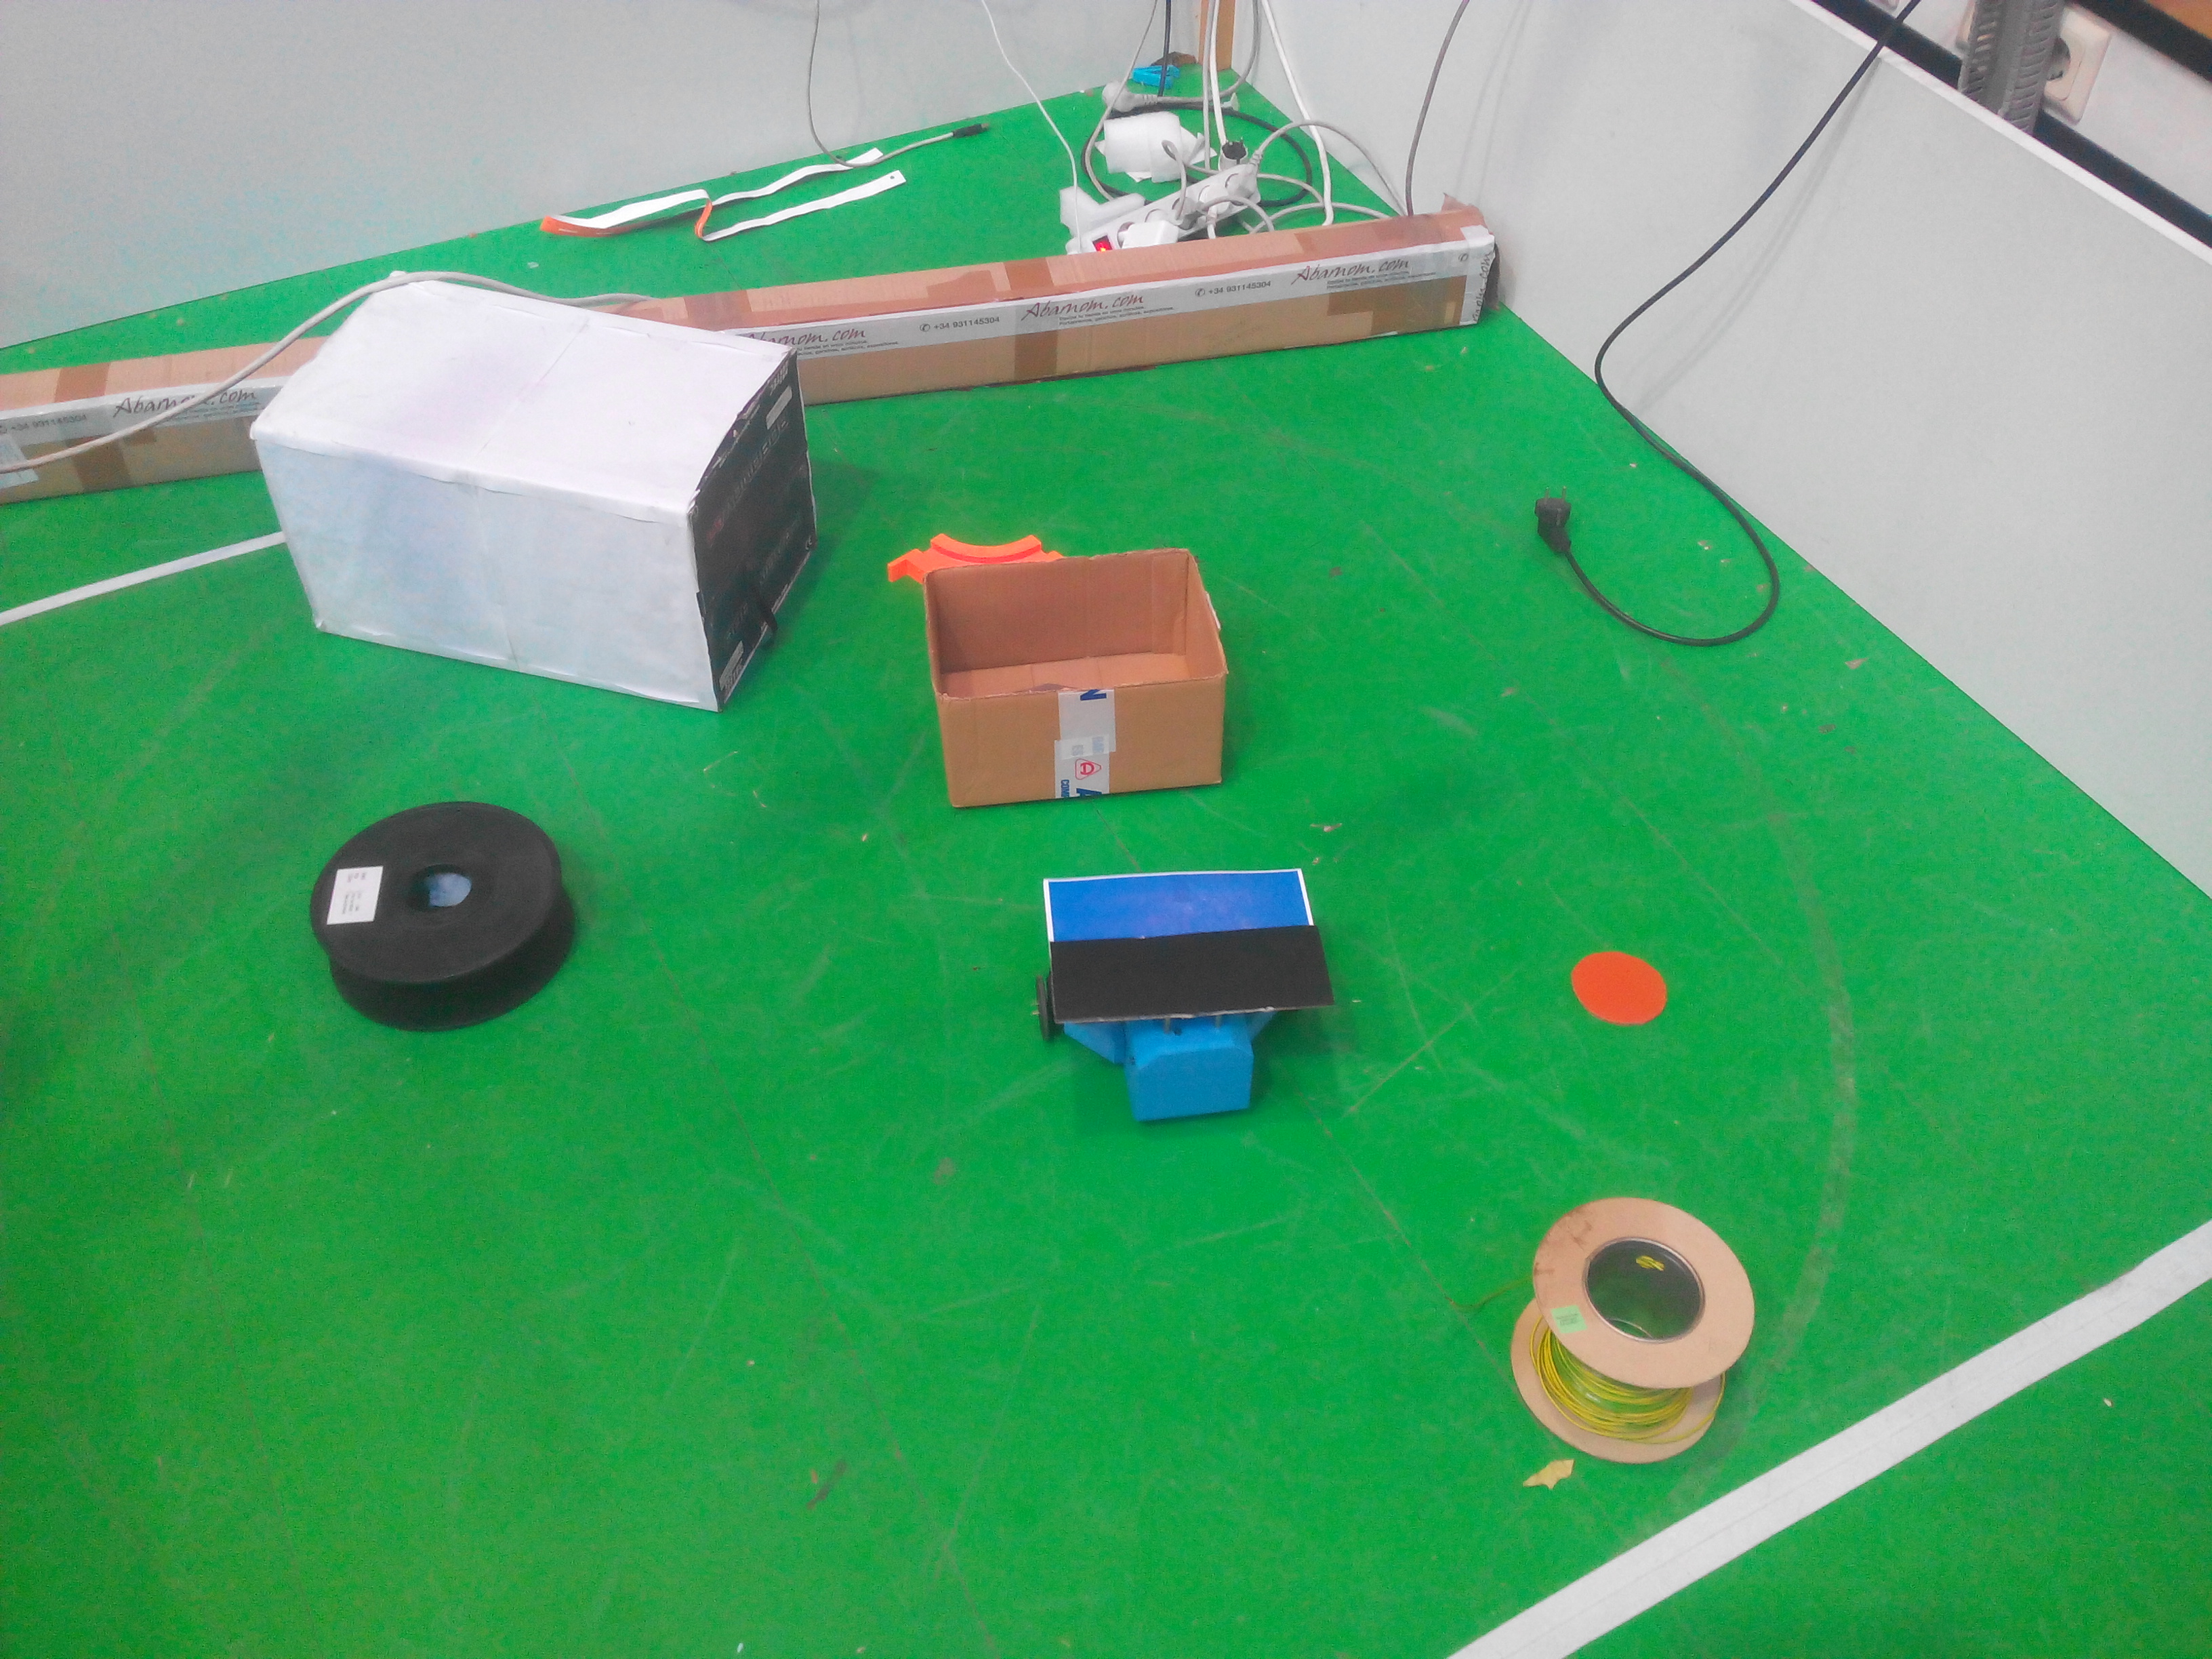
\includegraphics[width=0.5\textwidth]{images/environment_without_david.jpg}
        \caption{Escenario empleado}
        \label{fig:escenario}
\end{figure} 

Esta solución presenta varios problemas, siendo uno bastante importante las vibraciones que se generan al temblar el cable. Esto se podría solucionar fabricando una estructura rígida que soporte mejor la cámara. Otro problema por utilizar este escenario, quizás el más grave de todos, es que está situado en una zona muy amplia que, a pesar de ser interior, recibe una gran cantidad de luz natural proveniente de grandes ventanas situadas en el techo, que unido a la luz artificial presente, provoca que no se consiga una iluminación constante a lo largo del día, generándose gran cantidad de sombras en algunas zonas, o brillos en otras (esto también se debe al tipo de suelo que presenta el entorno), lo que dificulta en gran medida el correcto procesamiento de la imagen.\\  
\section{Hardware}
\label{hardware}


\subsection{Diseño mecánico}

El diseño del robot se ha realizado mediante el programa FreeCAD. FreeCAD, es un programa de modelado 3D paramétrico. El motivo fundamental de haber utilizado FreeCAD, es que es un programa libre. Para realizar el diseño mecánico del robot, se han tenido en cuenta los siguientes requisitos:

\begin{itemize}
	\item El robot tendrá una configuración diferencial.
	\item Poseerá una pinza que le permita recoger latas.
	\item Sus piezas deberán tener el tamaño adecuado para poder ser fabricadas en una impresora 3D de escritorio.
\end{itemize}

Siguiendo estos puntos, se ha diseñado un chasis con dos ruedas laterales. El tercer punto de apoyo se ha conseguido utilizando una canica. En la figura \ref{fig:abajo} se muestra una imagen del robot visto desde abajo, pudiendo observarse la colocación de las ruedas y de la caníca en el chasis.

\begin{figure}[H]
        \centering
        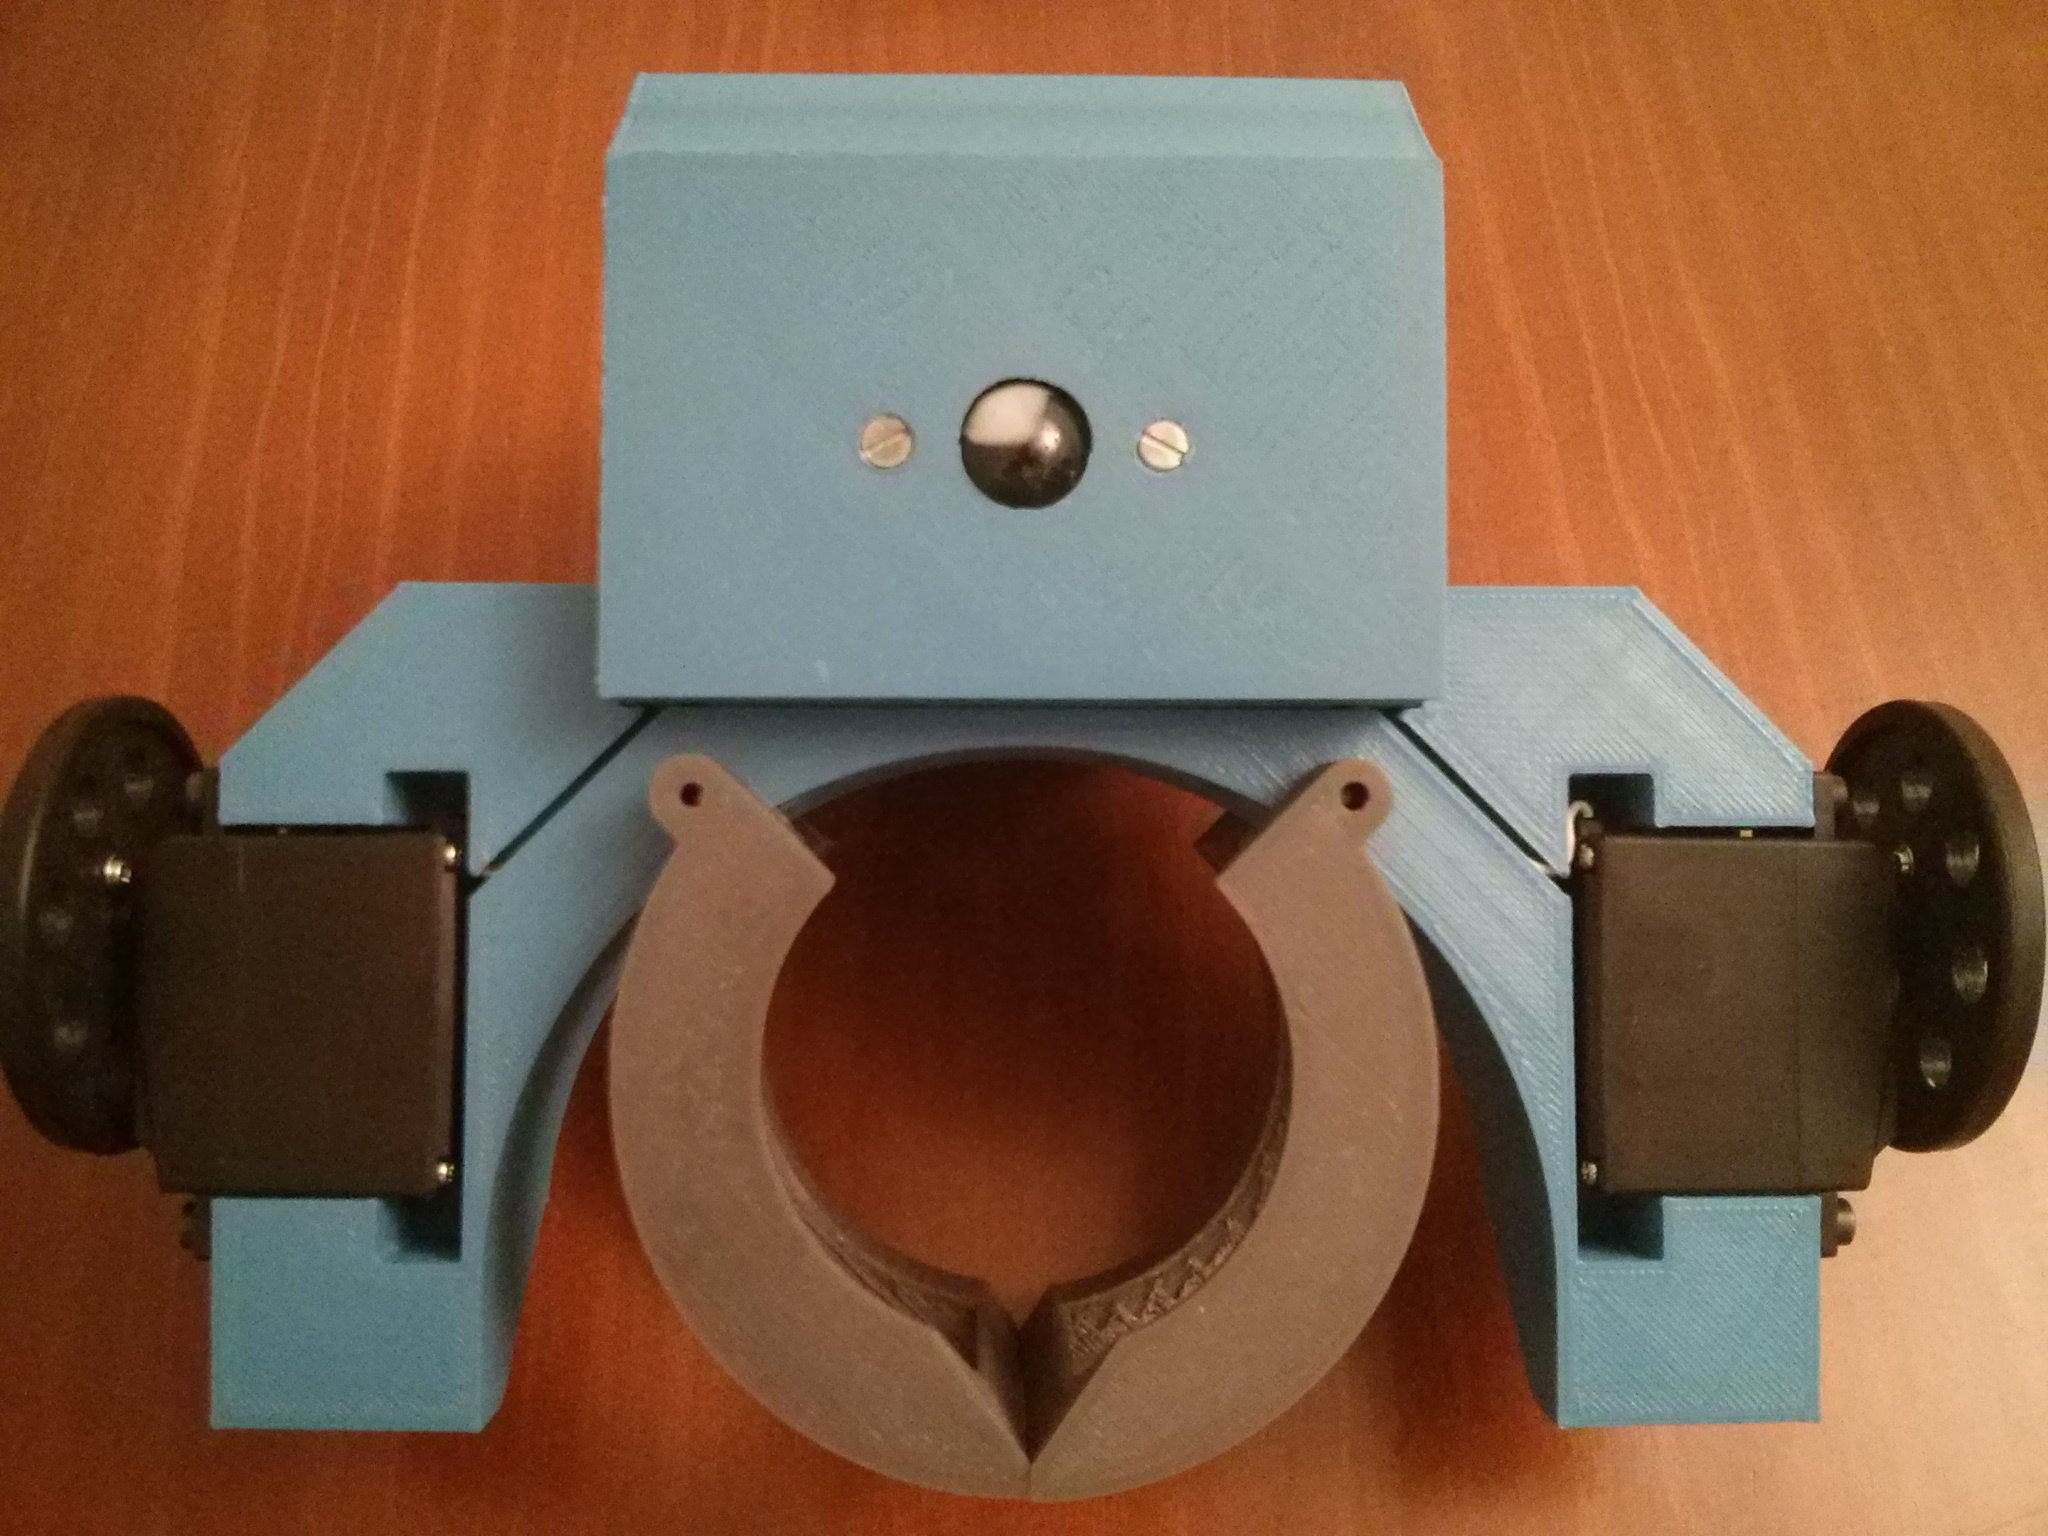
\includegraphics[width=0.4\textwidth]{images/abajo.jpg}
        \caption{Vista inferior del Beerbot}
        \label{fig:abajo}
\end{figure} 
El chasis, sirve de soporte para la pinza, la cual se actuará mediante un sistema de rótulas esféricas que transmitirán el movimiento desde un servomotor. Este sistema, además de presentar una gran robustez, permite controlar de manera precisa el rango de apertura de la pinza. Dado que la pinza cumplirá únicamente la función de agarrar latas, se ha diseñado un saliente en su parte inferior que permite elevar las latas ligeramente en el momento de agarrarlas. Gracias a esto, la lata no rozará contra el suelo y el robot podrá moverse libremente. El resultado puede observarse en la figura \ref{fig:pinza}.

\begin{figure}[H]
        \centering
        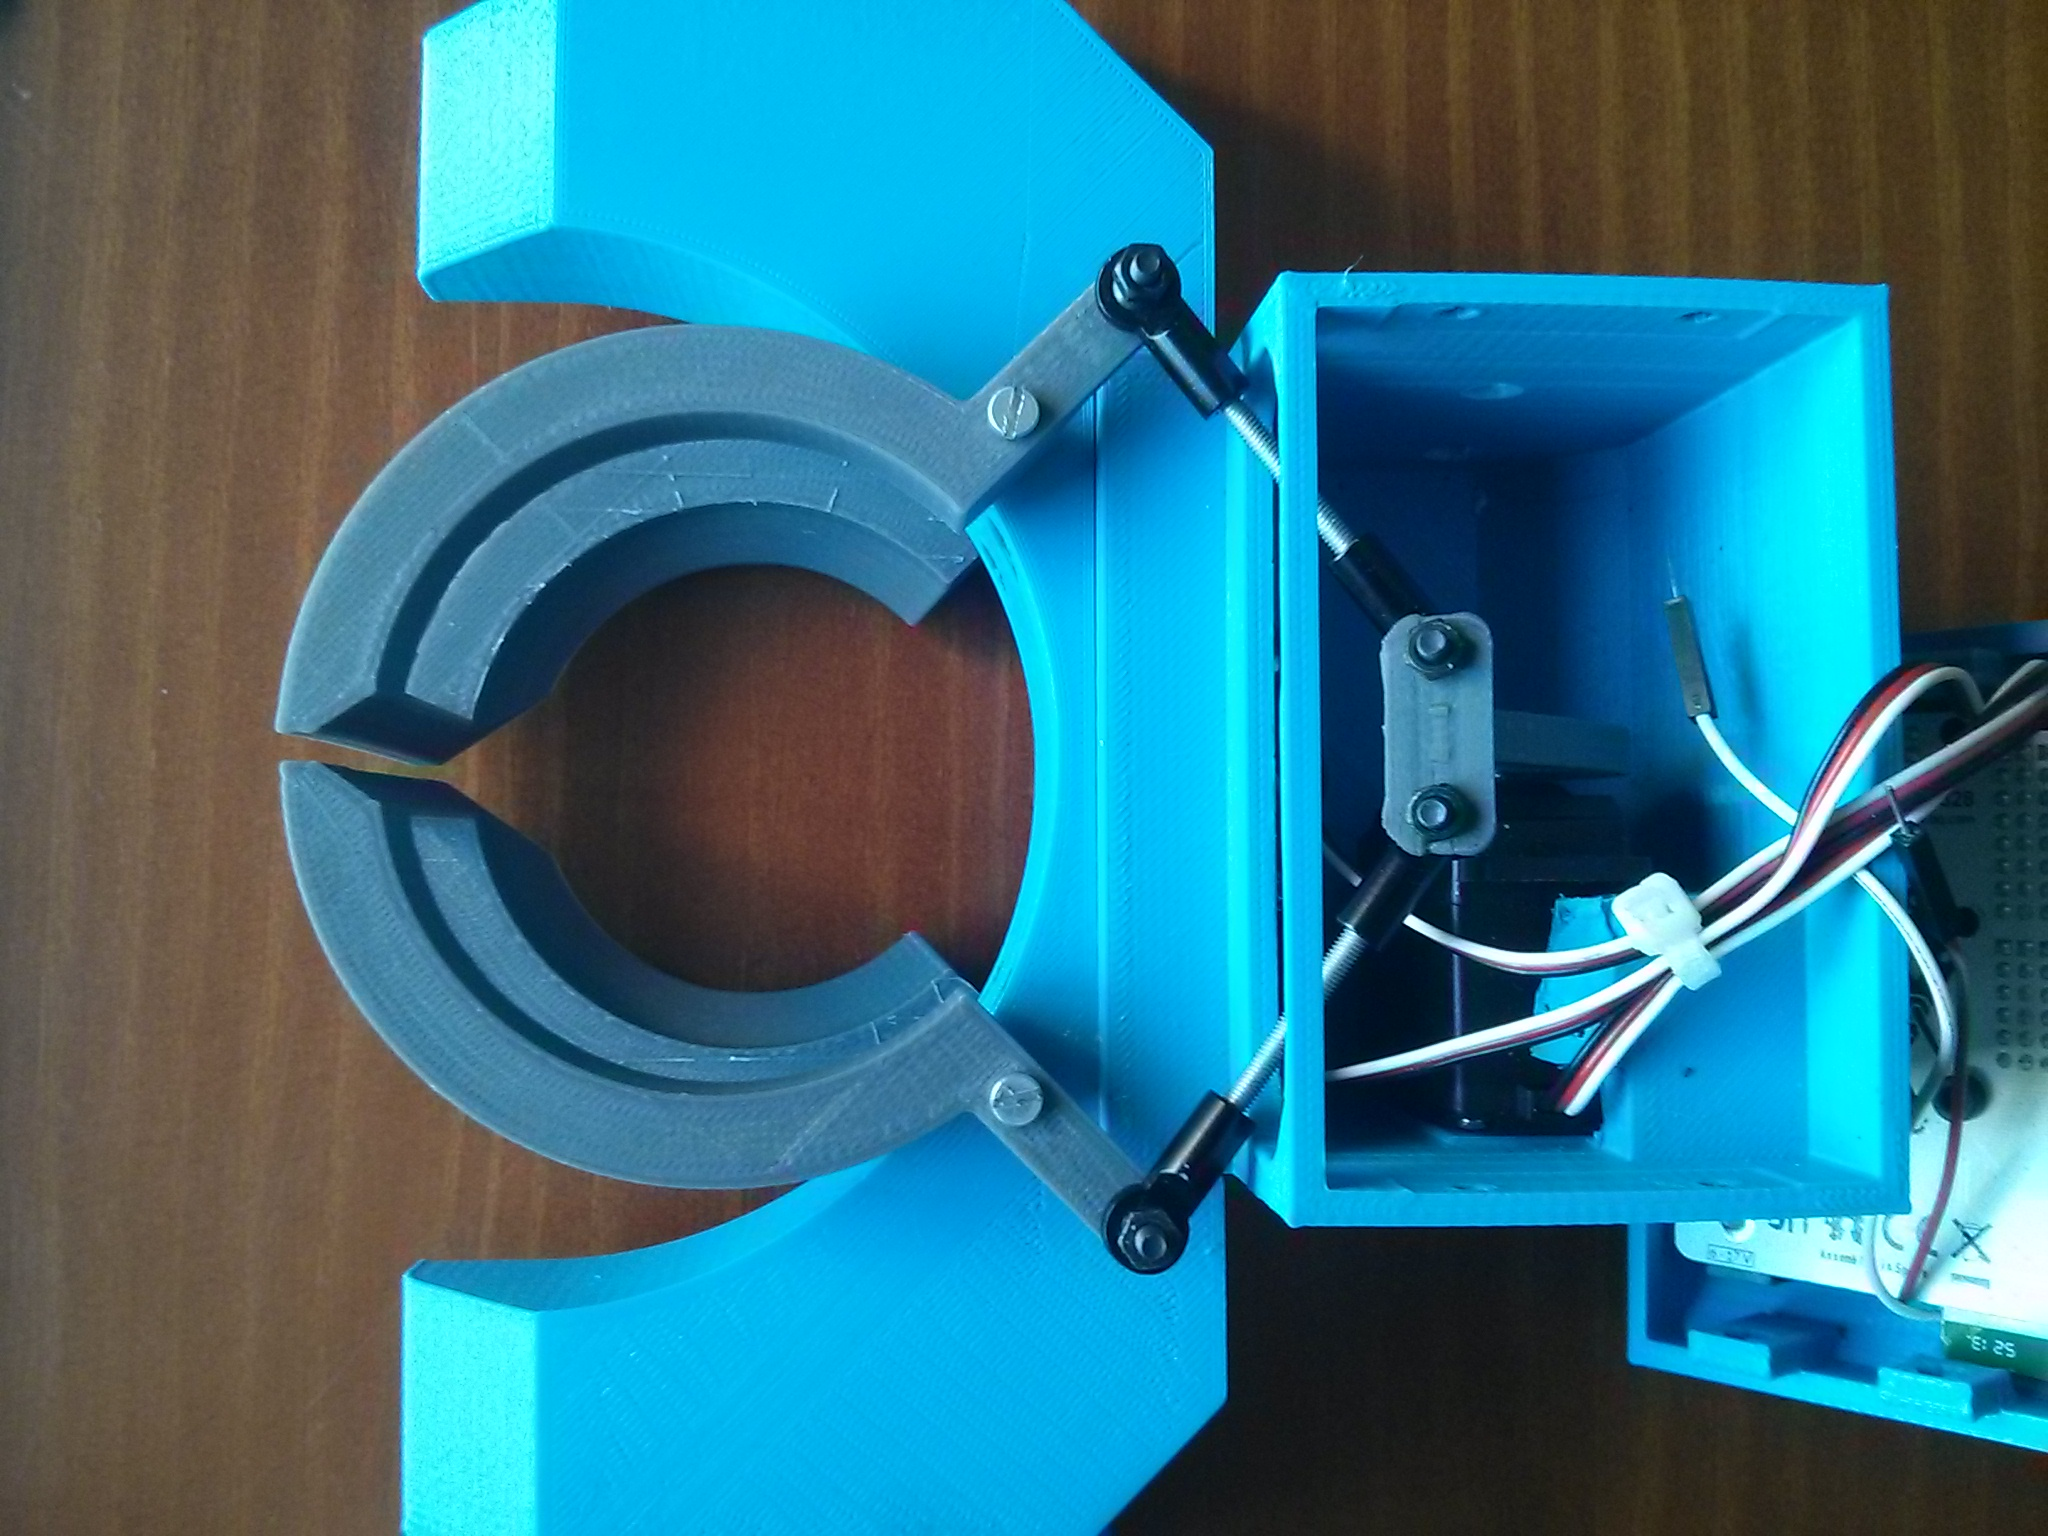
\includegraphics[width=0.4\textwidth]{images/pinzacerrada.jpg}
        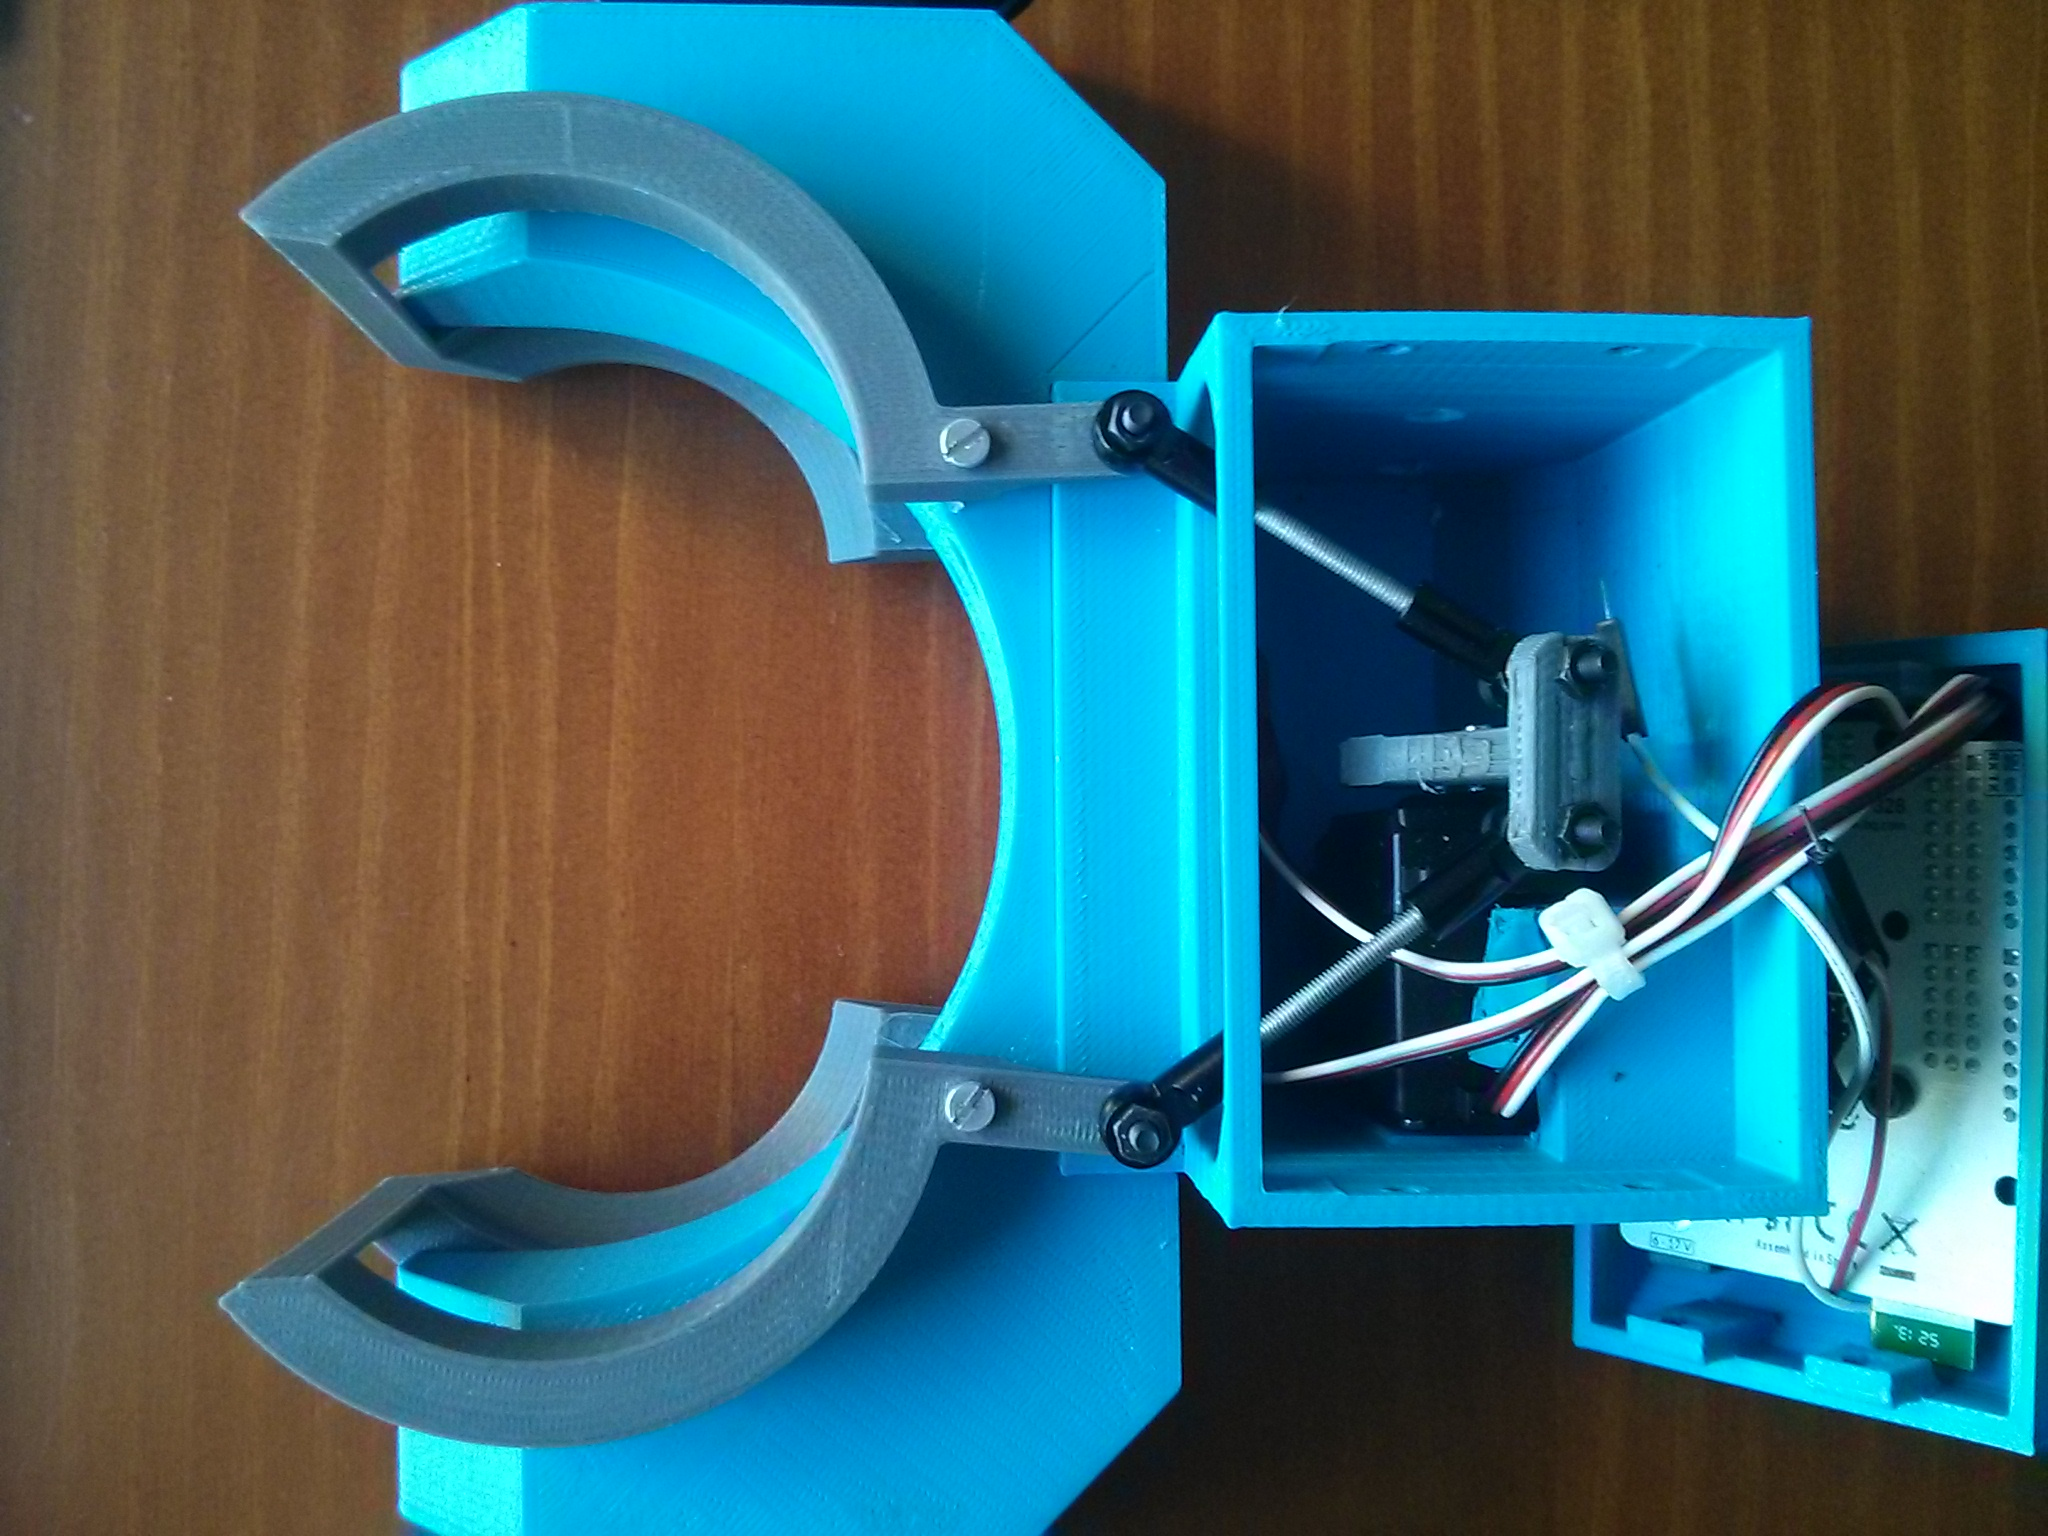
\includegraphics[width=0.4\textwidth]{images/pinzaabierta.jpg}
        \caption{Apertura de la pinza}
        \label{fig:pinza}
\end{figure} 
Se han diseñado un total de ocho piezas para montar el robot. Ninguna de ellas excede en planta una superficie de 20x20cm, lo que las hace imprimibles en la mayoría de las impresoras 3D de escritorio. En este caso particular, las piezas han sido impresas en un impresora BQ Witbox. El resultado final puede observarse en la figura \ref{fig:beerbot}

\begin{figure}[H]
        \centering
        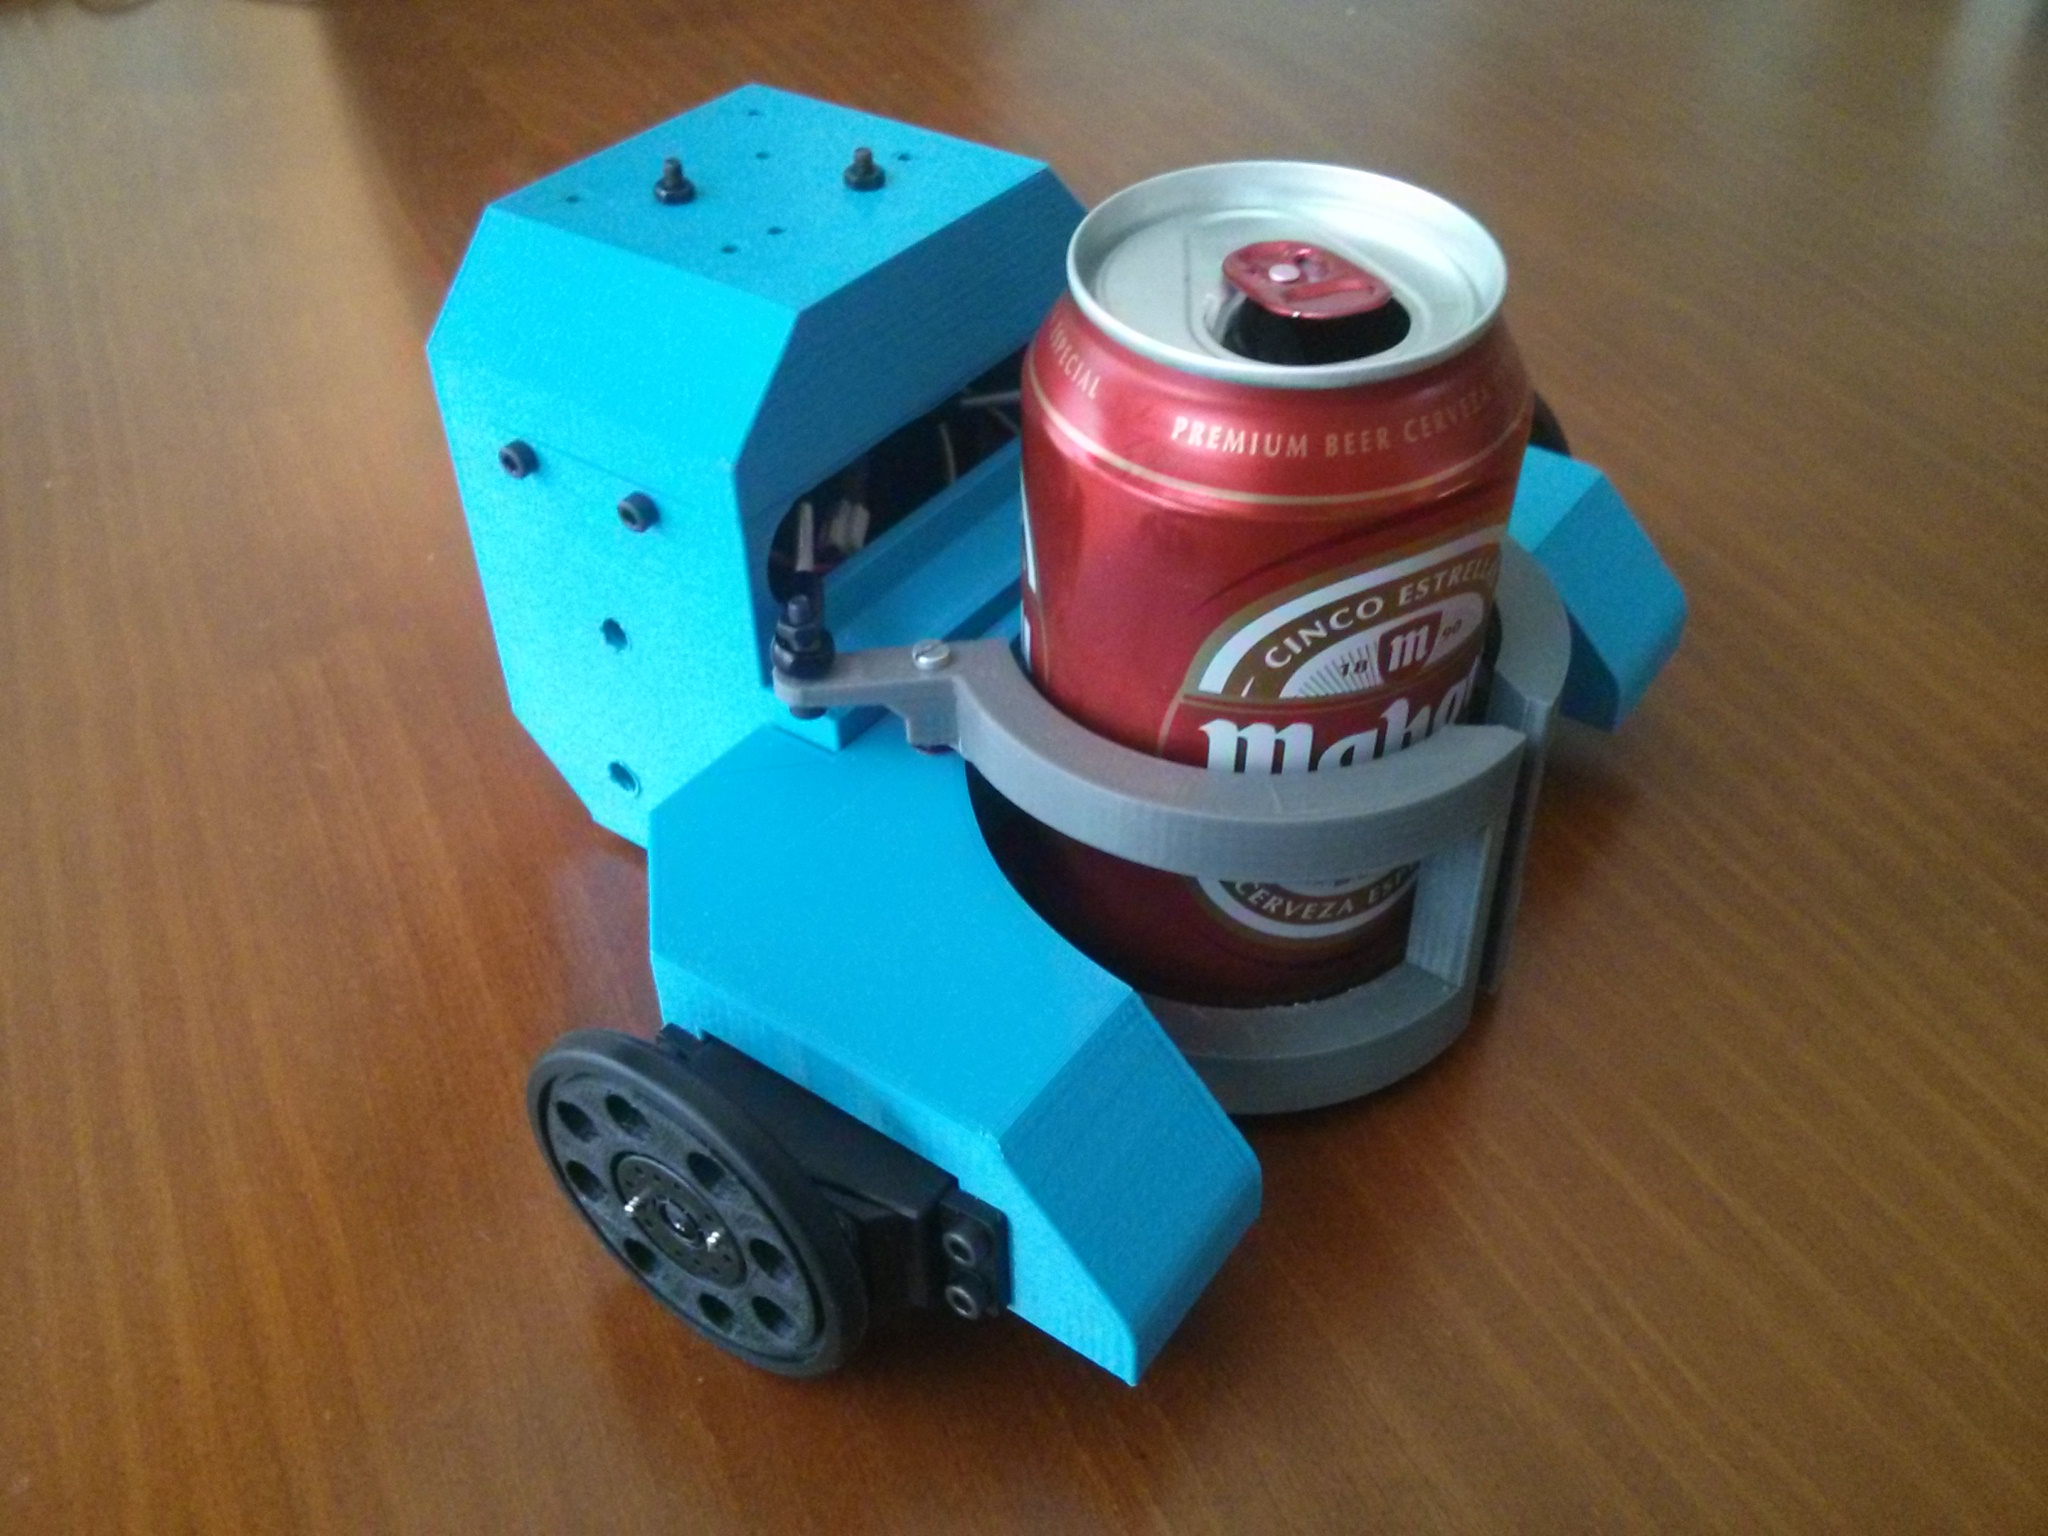
\includegraphics[width=0.4\textwidth]{images/beerbot.png}
        \caption{Beerbot ensamblado}
        \label{fig:abajo}
\end{figure} 

\subsection{Electrónica}

El robot utiliza un controlador BQ ZUM. Esta placa está basada en el microcontrolador ATmega328. La decisión de utilizar esta placa radica en que incluye un módulo Bluetooth, así como un sistema de alimentación que permite conectar directamente a la placa los motores del robot. En la figura \ref{fig:zum} puede observarse una placa BQ ZUM.

\begin{figure}[H]
        \centering
        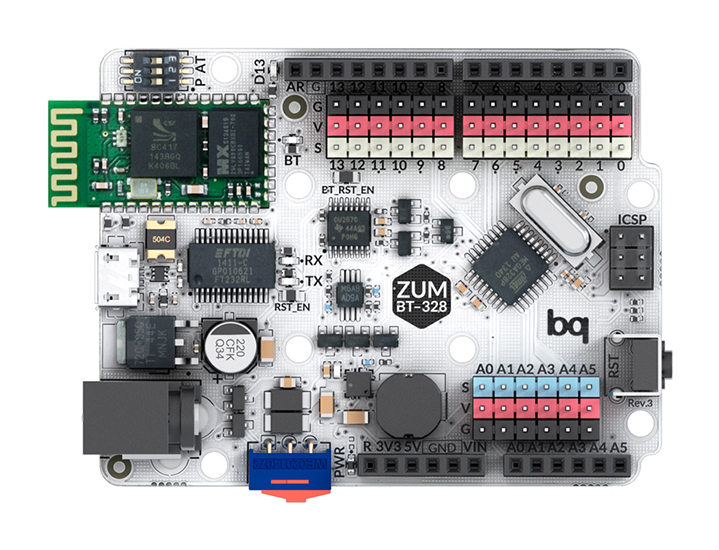
\includegraphics[width=0.4\textwidth]{images/zum.jpg}
        \caption{Placa controladora BQ ZUM}
        \label{fig:zum}
\end{figure} 

Para mover las ruedas del robot, se han utilizado dos servos de tamaño estándar de la marca Futaba, cómo el mostrado en la figura \ref{fig:futaba}. Estos servos han sido modificados para que rotasen de forma continua inutilizando el potenciómetro interno. El motivo de utilizar servos en vez de motores de corriente continua es principalmente el precio, la facilidad de controlarlos y que son fáciles de encontrar en tiendas de radiocontrol. La modificación del servo nos permite pasar de controlar el giro en posición a controlarlo en velocidad. Adicionalmente, se ha utilizado otro servo (sin modificaciones) para controlar la pinza.

\begin{figure}[H]
        \centering
        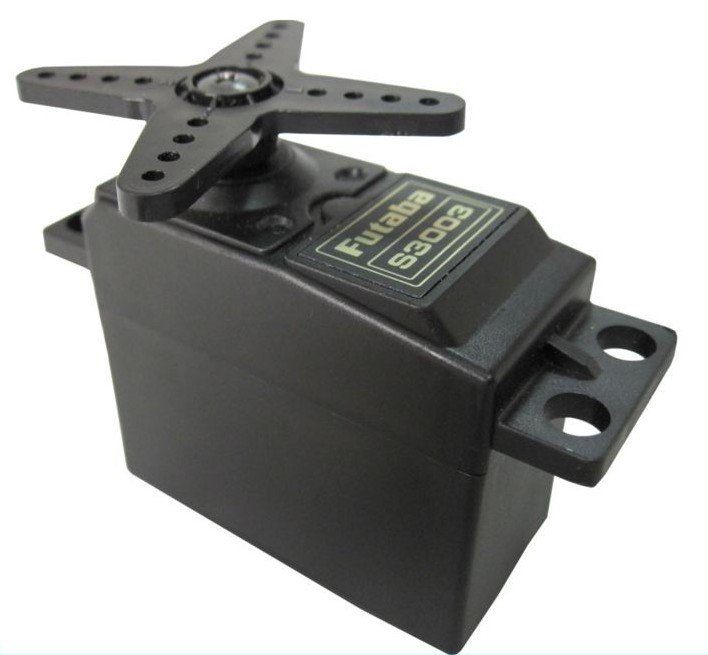
\includegraphics[width=0.4\textwidth]{images/futaba.jpg}
        \caption{Servo Futaba s3003}
        \label{fig:futaba}
\end{figure} 
En lo que a alimentación se refiere, se ha utilizado una batería de litio de dos celdas, con una tensión de 12V y una capacidad de 1000mAh. La autonomía del robot en constante movimiento es de aproximadamente 60 minutos. Dado que las pruebas realizadas no exceden los 5 minutos de duración, es una autonomía bastante razonable.

\subsection{Arquitectura del sistema}

El sistema completo, contará con tres elementos principales: el robot, una cámara y un ordenador. La cámara estará conectada al ordenador, el cual se comunicará a su vez con el robot de forma inalámbrica. En el esquema de la figura \ref{fig:arquitectura} se muestra la arquitectura completa del sistema.

\begin{figure}[H]
        \centering
        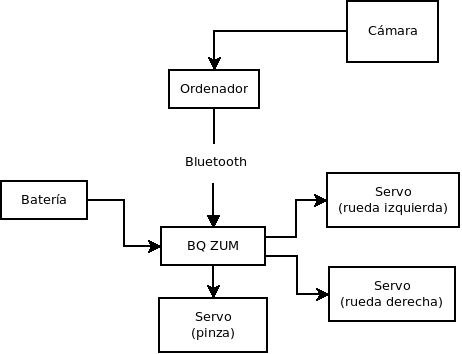
\includegraphics[width=0.6\textwidth]{images/arquitectura.jpg}
        \caption{Arquitectura hardware}
        \label{fig:arquitectura}
\end{figure} 
\section{Software}
\label{software}

\subsection{Calibración del sistema de visión}
\label{calibracion}
Para una correcta percepción del entorno es necesario realizar una calibración de la cámara para corregir las distorsiones producidas en la imagen por la lente y el sensor de la misma. La cámara posee dos tipos de distorsión: la radial, generada por la lente y que produce la curvatura de las líneas rectas de la imagen, y la tangencial, producida por un desalineamiento de la lente con el plano del sensor, de forma que ambos no se encuentran paralelos. La distorsión tangencial provoca que ciertas zonas de la imagen parezcan más cercanas de lo que realmente están.\\

Las fórmulas que modelan la distorsión radial son las siguientes:
\[x_{corrected} = x (1 + k_1 r^2 + k_2 r^4 + k_3 r^6)\]
\[y_{corrected} = y (1 + k_1 r^2 + k_2 r^4 + k_3 r^6)\]
~\\
 
La distorsión tangencial se modela con las siguientes fórmulas:
\[x_{corrected} = x + \left[2 p_1 x y + p_2 (r^2 + 2 x^2) \right] \]
\[y_{corrected} = y + \left[p_1 (r2 + 2 y^2) + 2 p_2 x y \right] \]
~\\

En total, la distorsión la modelaremos con 5 parámetros: $(k_1 ~ k_2 ~ p_1 ~ p_2 ~ k_3)$\\

También es necesario obtener los parámetros intrínsecos, que son propios de la cámara, como la distancia focal y el centro óptico, así como los parámetros extrínsicos de la cámara,posición y orientación respecto de un sistema de coordenadas 3D.\\

La matriz de la cámara expresa estos parámteros intrínsecos en una sola matriz:
\[camera ~matrix = \begin{bmatrix} f_x & 0 & c_x \\ 0 & f_y & c_y \\ 0 & 0 & 1 \end{bmatrix}\]
Donde $(f_x, f_y)$ son las distancias focales en los ejes x e y, y  las coordenadas del centro óptico son $(c_x, c_y)$.\\

Para realizar la calibración de la cámara es necesario un patrón de calibración como el de la figura \ref{fig:patron_calibracion}, de dimensiones conocidas. Las bibliotecas OpenCV poseen funciones capaces de reconocer y detectar automáticamente los vértices de los cuadrados y, conociendo su posición dentro del patrón y las dimensiones del mismo en la realidad, calcular los parámetros de la cámara.\\

\begin{figure}[H]
        \centering
        
\includegraphics[width=0.5\textwidth]{images/pattern.png}
        \caption{Patrón de calibración proporcionado por OpenCV}
        \label{fig:patron_calibracion}
\end{figure} 

El proceso es el siguiente. En primer lugar se coloca la cámara fija y se realizan una serie de fotos del patrón de calibración en distintas posiciones y orientaciones. Se extraen de estas imágenes los puntos correspondientes a los vértices de los cuadrados del patrón (figura \ref{fig:deteccion_patron}), que OpenCV usa para calcular tanto los parámetros de la distorsión como los parámetros intrínsecos de la cámara.\\

\begin{figure}[H]
        \centering
        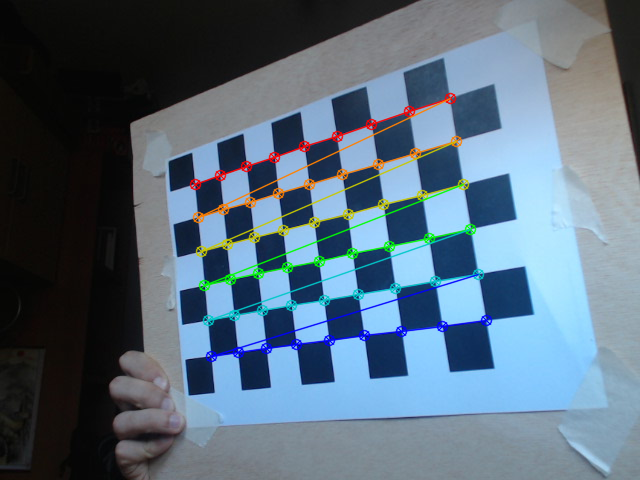
\includegraphics[width=0.5\textwidth]{images/calibration_pattern_detected.png}
        \caption{OpenCV detectando el patrón de calibración}
        \label{fig:deteccion_patron}
\end{figure} 

Una vez obtenidos estos parámetros, se almacenan en un archivo de forma que puedan ser cargados posteriormente. Usando estos archivos, es posible rectificar la imagen para eliminar la distorsión usando la función undistort de OpenCV, y posteriormente se recorta la región de interés de la imagen.\\



\subsection{Procesamiento del entorno}
\label{procesamiento}

El primer paso del algoritmo de planificación y control es la extracción de información del entorno a través de visión artificial. Al no poseer ningún tipo de sensor, toda la información que posee el controlador del robot se obtiene a través del sistema de visión.\\

\begin{figure}[H]
        \centering
        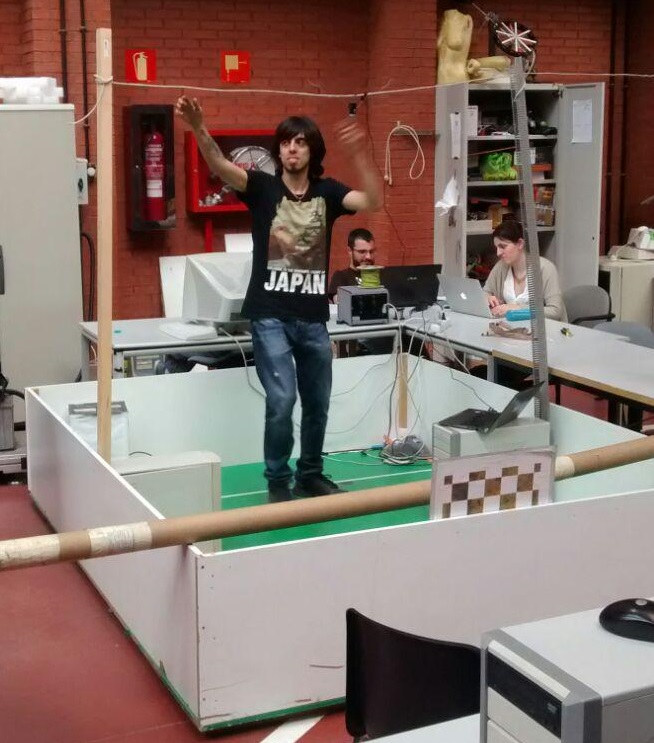
\includegraphics[width=0.4\textwidth]{images/escenario.jpg}
        \caption{David colocando la estructura de soporte de la cámara cenital}
        \label{fig:foto_estructura_nave}
\end{figure} 

El entorno es captado a través de una cámara cenital, fijada a una estructura de soporte (figura \ref{fig:foto_estructura_nave}). El suelo del entorno, un escenario del concurso CEABOT, está pintado de un llamativo tono de verde. Para su localización, el robot lleva en su parte superior un marcador fiduciario formado por un rectángulo de dos colores, negro y azul (figura \ref{fig:marcador_fiduciario}). Al poseer dos colores es posible extraer tanto la posición como la orientación del robot a través de la cámara.\\

\begin{figure}[H]
        \centering
        
\includegraphics[width=0.4\textwidth]{images/marcador.png}
        \caption{Marcador fiduciario usado para el tracking del robot}
        \label{fig:foto_estructura_nave}
\end{figure} 

Para la detección de obstáculos se utiliza una segmentación del color verde, aplicando una umbralización en el espacio de color HSV. La máscara resultante se procesa con una apertura usando un kernel rectangular de 5x5 píxeles, para reducir el ruido, y se lleva a cabo un etiquetado de objetos sobre la imagen binaria filtrada. Estos contornos, posteriormente, son también filtrados por tamaño y área, y simplificados.\\

A partir de los contornos de estos obstáculos se genera una imagen binaria que es utilizada como mapa para el algoritmo de planificación (figura \ref{fig:map}).\\

\begin{figure}[H]
        \centering
        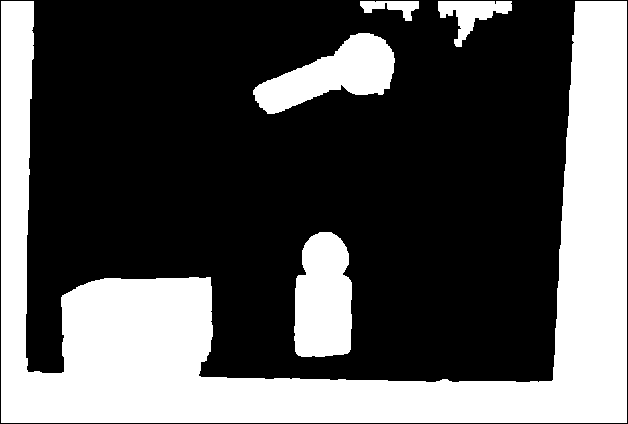
\includegraphics[width=0.4\textwidth]{images/map.png}
        \caption{Mapa del entorno obtenido a partir de los contornos de los obstáculos segmentados.}
        \label{fig:foto_estructura_nave}
\end{figure} 

El marcador del robot se extrae mediante una segmentación del color azul, llevada a cabo también umbralizando en el espacio HSV y realizando el mismo filtrado que en el caso del color verde. Para una detección robusta del color negro del marcador, y para evitar reflejos producidos por una iluminación no controlada, el marcador completo se detecta buscando entre los obstáculos detectados el que posea un rectángulo azul en su interior, que es identificado y etiquetado como robot.\\ 

La posición del robot se obtiene calculando el centro del contorno del robot, y la orientación usando el vector que conecta el centro de dicho contorno con el centro del contorno azul, midiendo su orientación con respecto al eje X.\\

Por último, para la detección de la lata, se comprueban todos los obstáculos buscando aquellos que tengan forma circular. Esta forma circular se calcula teniendo en cuenta la proporción entre el área del contorno y el área del menor circulo que incluye el contorno, que es aproximadamente 1 en el caso de que el contorno sea totalmente circular. Para que la segmentación no etiquete obstáculos circulares como latas, se realiza también un filtrado de candidatos por tamaño, reduciendo así el número de posibles falsos positivos.\\

La figura \ref{fig:segmentation} muestra el resultado de la segmentación. Los contornos amarillos indican los obstáculos, los círculos azules son las latas (objetivos) detectadas y el rectángulo magenta rodea al robot, cuya orientación queda indicada con una línea cyan.\\

\begin{figure}[H]
        \centering
        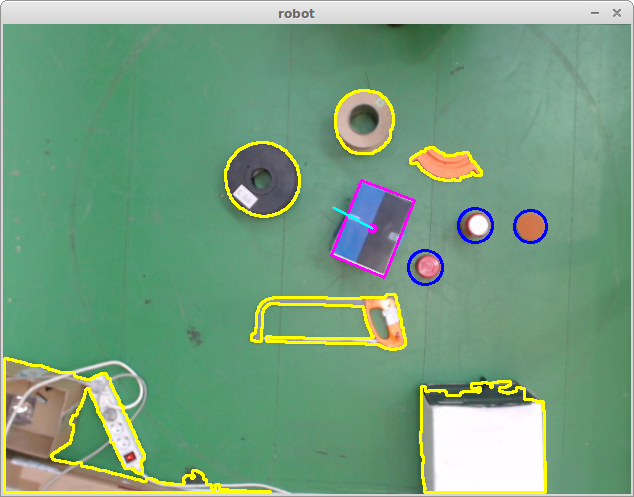
\includegraphics[width=0.4\textwidth]{images/segmentation.png}
        \caption{Resultado de la segmentación}
        \label{fig:segmentation}
\end{figure} 
\subsection{Planificacion de trayectorias}
\label{planificacion}
\subsection{Control del robot y seguimiento de la trayectoria}
\label{control}

El control a más bajo nivel se ha realizado variando la velocidad de los motores del robot. Como se comentó en el apartado de hardware, los motores del robot se han obtenido al modificar servos. Los servos de radiocontrol se controlan mediante señales PWM. La posición de los servos se controla mediante la variación de la anchura de los pulsos. La electrónica del servo implementa un controlador PID y gracias a este controlador podremos conseguir controlar el servo en velocidad. El método para lograrlo consiste en buscar los valores de la PWM que generan posiciones próximas a la posición que marca el potenciometro del servo (como recordatorio, al modificar el servo este potenciómetro marcará siempre una posición constante y no variará cuando varíe el giro del motor). Cuando al servo se le pide una posición próxima a la medida por el potenciómetro, este girará de forma lenta. Sin embargo, cuando la posición se aleja de la medidad del potenciómetro la velocidad será mayor, hasta llegar a un punto de saturación. Experimentalmente, se ha definido un rango de aproximadamente 250 ms en el que la variación del ancho de pulso es lineal respecto a la velocidad.

Para enviar comandos de velocidad del ordenador al robot, se han codificado los valores de la PWM en un byte para cada rueda. Es decir, el rango efectivo de funcionamiento tomará valores desde -128 a 127, siendo el 0 el punto en el que el motor estará parado. Estos valores se enviarán por Bluetooth.

En este punto, se tiene un control del movimiento del robot en dos dimensiones, y mediante la cámara obtenemos realimentación de su posición y su orientación. Dado que el planificador ofrece una serie de puntos que hay que recorrer pra completar la trayectoria, solo resta implementar los controladores del robot para conquistar esos puntos.

El primer controlador implementado ha sido la función de giro y orientación. En nuestra aplicación, es muy importante realizar giros controlados, ya que repercutirán con gran importancia en la suavidad de los movientos del robot, así como en el tiempo ocupado en realizar la prueba. Por una parte, se requiere conocer en todo momento la orientación del robot respecto al eje de coordenadas de la imágen. Al mismo tiempo, el controlador debe permitir modificar esta orientación con el objetivo de dirigir el robot correctamente hacia los puntos. A continuación, en la figura \ref{fig:flujogiro} se muestra un diagrama de estados en el que se define el modo de actuación del robot tras una orden de giro.\\

\begin{figure}[H]
		\centering
        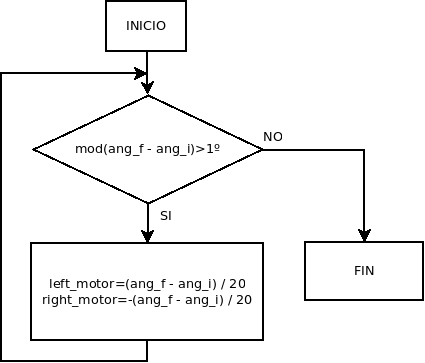
\includegraphics[width=0.5\textwidth]{images/flujogiro.png}
        \caption{Diagrama de estados del controlador de giros}
        \label{fig:flujogiro}
\end{figure} 

El segundo controlador del robot corresponde a su traslación. Ya que el robot constituye el punto de inicio de cualquier trayectoria que sea desarrollada, se debe conocer su posición inicial antes de correr el algoritmo de planificación. También, durante el experimento, se requiere un conocimiento en tiempo real de la posición global del robot. Este controlador nos permitirá definir el desplazamien y la consecución de objetivos del robot. En el siguiente diagrama de estados, representado en la figura \ref{fig:flujoavance}, se muestra la implementación de este controlador.

\begin{figure}[H]
		\centering
        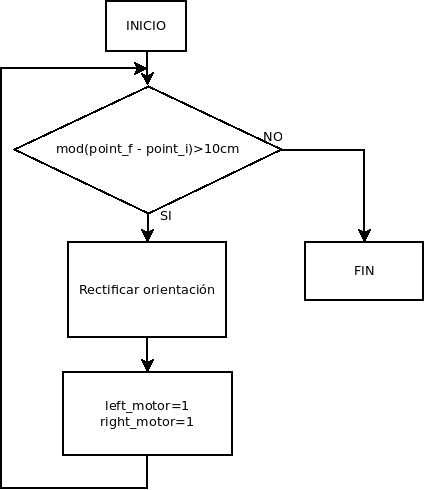
\includegraphics[width=0.5\textwidth]{images/flujoavance.png}
        \caption{Diagrama de estados del controlador de desplazamiento}
        \label{fig:flujoavance}
\end{figure} 
\chapter{Resultados obtenidos y futuras mejoras}
\label{resultados}

En esta sección se van a comentar los resultados extraídos del proyecto Beerbot. Se debe comenzar comentando que, en última instancia, el trabajo resultó un éxito completo, ya que se alcanzaron los objetivos que se habían planteado. El robot fue capaz de desplazarse por el entorno evitando los obstáculos sin problemas y alcanzando el objetivo asignado. Para poner a prueba el funcionamiento del sistema, se desarrollaron tres escenarios distintos, variando la distribución de los obstáculos. Estos se pueden observar en la figura \ref{escenarios}.\\

\begin{figure}[h]
		\centering
        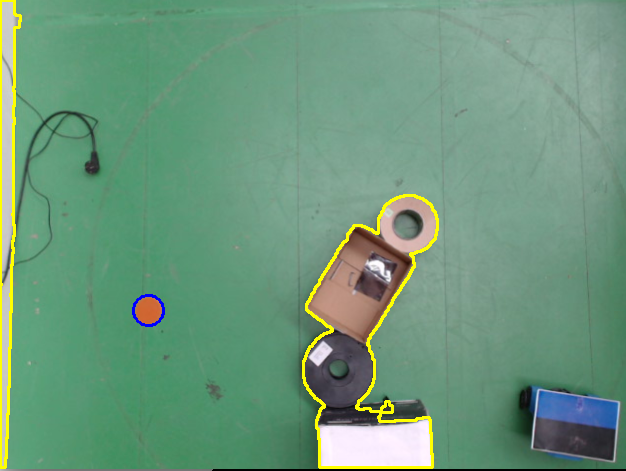
\includegraphics[width=0.35\textwidth]{images/configuration1_segmented.png}
        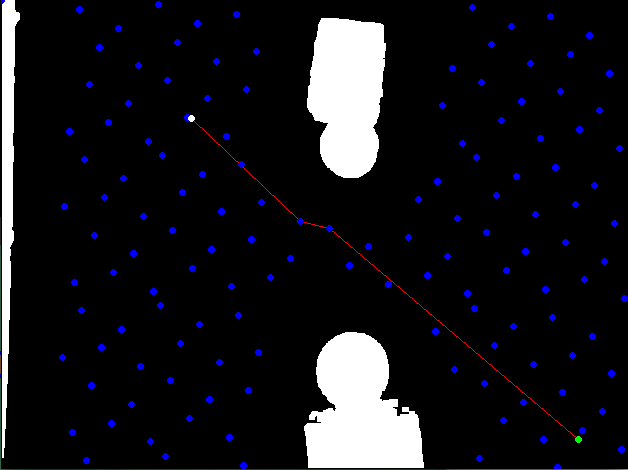
\includegraphics[width=0.35\textwidth]{images/configuration2_trajectory.png}
        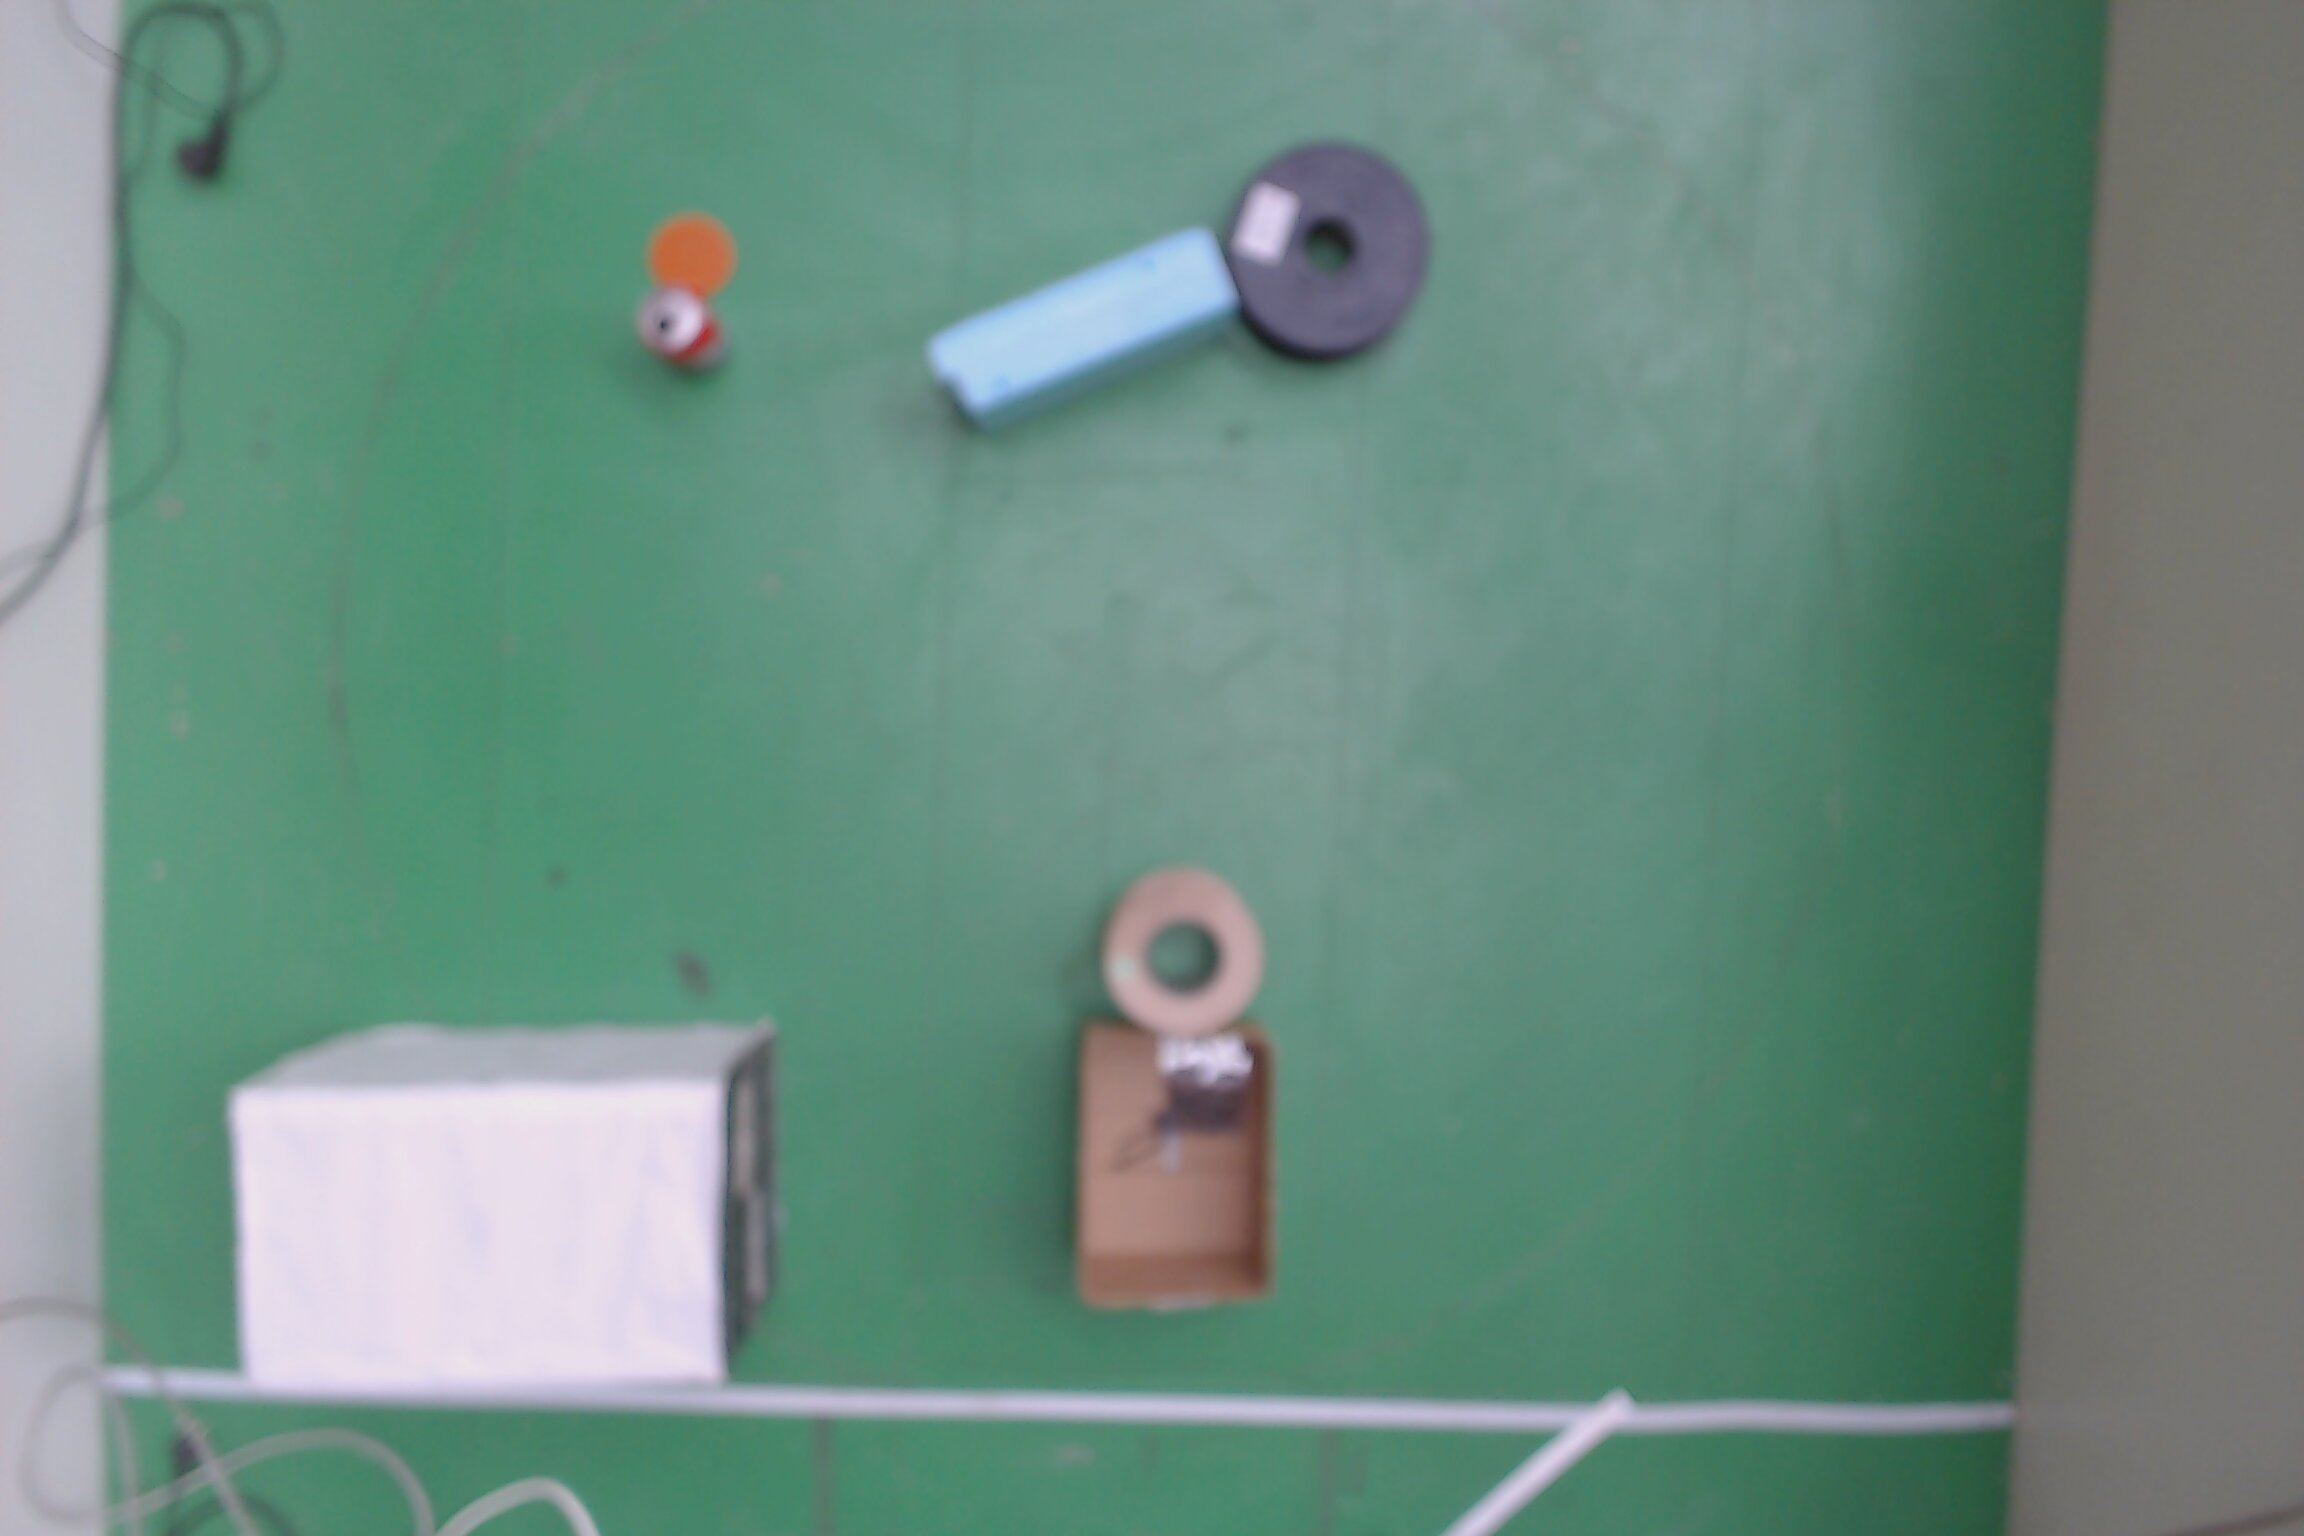
\includegraphics[width=0.35\textwidth]{images/configuration_3.jpg}
        \caption{Escenarios empleados}
        \label{escenarios}
\end{figure}

En los tres entornos el robot fue capaz de alcanzar el punto final sin problemas. Además, se probó a variar la velocidad de avance y se comprobó que, aunque seguía funcionando, pdía dar algunos problemas, ya que el sistema necesita pasar por los puntos definidos. ÇEn caso de saltarse alguno, el robot se dará la vuelta, irá hasta el nodo que se ha saltado y luego continuará con el camino. En todo caso, este no es un problema fatal, ya que se sigue llegando al lugar deseado, solo supone una cierta perdida de tiempo. El único caso en el que el robot no fue capaz de alcanzar el objetivo se dió cuando la trayectoria se acercaba demasiado al límite de la imagen que se capta con la cámara. Si el robot en este caso se desvía de la trayectoria y se sale de la zona controlada, pierde la localización, y se queda dando vueltas sobre si mismo. Esto se puede arreglar moviendo manualmente el robot de nuevo a la zona de trabajo.

A continuación se comentará como ha funcionado cada una de las partes del sistema en si. Respecto a la parte de procesamiento, inicialmente se planteó de forma distinta a como se ha implementado en la versión final. Se realizaba de igual manera una segmentación del color verde, que corresponde al suelo, en el espacio HSV. A esto se le añadía una segmentación de los colores azul y negro, para eliminar el robot, y del color rojo, para eliminar la lata. La imagen binaria resultante se enviaba al algoritmo de planificación, que se encargaba de extraer los obstáculos y demás. Para la posición y orientación de la lata se segmentaban los colores azul y negro, para encontrar el marcador del robot, y se calculaban los centros de ambas regiones y del marcador en si. Con este último se obtenía la posición del robot, con la orientación del marcador se extraía la dirección de movimiento y con los centros de ambas secciones se extraía el sentido en el que miraba el robot. Cuando esto se llevó a la práctica, se observó que su funcionamiento no era demasiado bueno, ya que los cambios de iluminación provocaban que las segmentaciones no diesen los resultados esperados. Aunque se consiguió filtrar de forma correcta los colores verde, azul y rojo, el color negro fué un problema constante, por lo que se decidió optar por otro enfoque, pasando a la solución explicada en el apartado de software de esta memoria. Con esto se consiguió hacer funcionar de forma adecuada el procesamiento de la imagen.\\

En cuanto al algoritmo de planificación, basta decir que cumplió con su cometido de forma correcta desde el primer momento, al ser un método desarrollado y probado previamente. En este caso no se han hecho estudios en profundidad acerca de como los distintos parámetros del algoritmo afectan a su funcionamiento, pero en caso de estar interesado, dichos estudios se pueden consultar en la memoria contenida en la librería  \textit{PLATANO} \footnote{https://github.com/JavierIH/platano}.\\

Por último, con respecto al sistema de control, fue necesaria una etapa de ajuste durante el proceso de pruebas para conseguir que todo funcionase como es debido. Los principales problemas que se encontraron fueron debidos a los problemas para extraer la orientación del robot debido a la iluminación irregular, que llevaba a una mala segmentación. Al no extraer de forma correcta la orientación, el controlador trataba de reorientar al robot de forma continua y no era capaz de avanzar. Sin embargo, ajustando la parte de procesamiento de la imagen se consiguió solucionar esto y se consiguió hacer navegar al robot sin más problemas que los ya comentados acerca de la perdida de localización si este se salía de la zona que capta la imagen y la necesidad de pasar por todos los puntos.\\

Como posibles mejoras al sistema, se ha pensado en dotar al robot de sensores para ser capaz de detectar y evitar obstáculos de forma reactiva, lo que podía ser útil en caso de que un mal ajuste pueda llevar a generar una trayectoria que pase demasiado cerca de un obstáculo. Además de esto, se podría variar el sistema de seguimento de la trayectoria para permitir un movimiento de avance continuó, mientras se va regulando la orientación del robot. Estó permitiría reducir el tiempo que se tarda en alcanzar el objetivo. Por último, si se consigue optimizar los tiempos de procesamiento del entorno y de planificación de trayectoria, se podría utilizar este sistema en entornos donde existiesen obstáculos no estáticos, comprobando cada cierto tiempo si la posición del obstáculo interfiere con la ruta planificada y buscando otro camino en caso de que esto suceda.\\  
\chapter{Conclusión}
\label{conclusion}

Con este trabajo se pretendía desarrollar una aplicación acerca de robots móviles. Después de haber repasado todos los aspectos del proyecto, la principal conclusión que se puede extraer de este es que los objetivos planteados se han cumplido en su totalidad. Se ha conseguido implementar un algoritmo de planificación que trabaja junto a un algoritmo de procesamiento de imágenes para poder adquirir la información del entorno.\\

El robot ha sido capaz de alcanzar el punto final y recoger la lata, evitando los obstáculos presentes en el entorno. Como todos los métodos de planificación basados en el muestreo, este sistema mejora su capacidad de encontrar una trayectoria si se incrementa el número de nodos. Tanto el Dijkstra como el $A^*$ son algoritmos completos, por lo que siempre van a encontrar un camino en caso de que exista. Esto se ha puesto a prueba y se ha confirmado experimentalmente. En cuanto al sistema de visión, se ha conseguido implementar un algoritmo que segmenta el entrono de forma bastante acertada, especialmente teniendo en cuenta que la iluminación deja bastante que desear. Por último, el diseño de robot ha sido totalmente adecuado para la tarea a resolver.\\

Como última conclusión, decir que se ha desarrollado un método robusto y funcional para conseguir mover el robot por un entorno con objetos estáticos. Como posibles mejoras, se podría mejorar el sistema de seguimiento de la trayectoria y el tiempo de procesamiento para poder aplicar este método a entornos dinámicos.\\

%%%% Appendices %%%%%%%%%%%%%%%%%%%%%%%%%%%%%%%%%%%%%%%%%%%%%%%%%%%%%%%%%%%%%
%\begin{appendices}

%\end{appendices}

%%%% Bibliography %%%%%%%%%%%%%%%%%%%%%%%%%%%%%%%%%%%%%%%%%%%%%%%%%%%%%%%%%%%%%
%\newpage
%\bibliographystyle{plain}
%\bibliography{Bibliography.bib}

\end{document}
